Although McG paper does not clearly state any results of the agents individually, this thesis aims to investigate the integrity of the implementation. This will be done by examining the agents' algorithm in detail, along with the specific parameters in addition to looking at cited papers in McG which relates to where the McG's agents are based from. The aim of this section is to ensure that if the system (the new BSE) and the agents themselves are performing like what they are meant to do, we can be certain that any experiment results from the market consisting of the agents will be valid. 


\section{Market maker}
The Market maker in McG is modelled closely to Oesch 2014 conference paper \cite{Oesch}. Market makers are traders who attempt to earn a profit by taking advantage of the spread in the market. The agent executes orders on both bid and ask side of the LOB in each round. The agent submits a large order with volume $V=U(v_{min},v_{max})$ depending on its moving average. The moving average is used to predict what type of orders will be submitted next. 

\begin{algorithm}[H]
\DontPrintSemicolon 
\If{$random() > \delta_{mm}$} {
    Cancel any existing order\;
    \tcc{Condition 1}
    \If{predict next order is buy} {
    \tcc{$U(a,b)$  function represents value drawn uniformly between $a$ and $b$ }
    Submit sell at best price with volume $V=U(v_{min},v_{max})$\;
    Submit buy at best price with volume $V=v^{-}$\;
    }
    \tcc{Condition 2}
    \Else{
    Submit buy at best price with volume $V=U(v_{min},v_{max})$\;
    Submit sell at best price with volume $V=v^{-}$\;
    }
    \EndIf
  }
\EndIf
Update buy/sell prediction with w-period rolling mean\; 
\caption{{\sc Market maker reproduced from McG (4.1) \cite{McGroarty}} }
\label{algo:market_maker}
\end{algorithm}

\begin{table}[h]
\centering
\begin{tabular}{ |m||p{4cm}|} 
\hline
\textbf{Market maker Parameters}& \textbf{Value} \\
\hline
\hline
$v_{min}$ & 100 \\ 
\hline
$v_{max}$ & 200,000\\ 
\hline
$v^-$ & 1\\ 
\hline
$w$ & 50\\
\hline
\end{tabular}
\caption{Market maker trader parameters taken from \cite{McGroarty} and  \cite{Oesch}} 
\end{table}
\FloatBarrier 

To clarify, the Market maker will make its decision based on a moving average of $w$ period. The moving average is calculated from the number of bids and asks in the $w$ period. In McG, the paper refers to Long Term memory order flow such that the future order is heavily correlated with the orders in the past. In each period, a buy order is given a +1 and a sell -1. The sum of those, if is negative, the Market maker agent will predict that an ask order will arrive next. This means that the agent will submit a bid large order with best price and quantity uniformly distributed from $U(v_{min},v_{max})$ and an ask order with quantity = $v^-$. This is Condition 1 on line 3 of Algorithm \ref{algo:market_maker}. Vice versa, if the sum of the period is positive as outlined in Condition 2 on line 6 of Algorithm \ref{algo:market_maker}. 

In order to test the Market maker behaviour, two simpler agents is implemented called Simple Buyer and Simple Seller. The Simple Buyer (Seller) will only submit a bid (an ask) order with price = $100$ in any circumstances with quantity uniformly distributed between 1 and 100. The total time period is 100 running with McG action step system. A short experiment is conducted where a market consisting of 6 Market makers and 6 of one of the Simple agents. The expected behaviour is that the Market maker will submit only an Ask order in a market with Simple Buyer since it will try to match the incoming bid orders. This is testing the first condition of the Algorithm \ref{algo:market_maker} where the Market maker will predict the next order is a buy. Vice versa for a market with Simple Seller. 

\begin{figure}[h]
  \begin{subfigure}[b]{0.5\textwidth}
    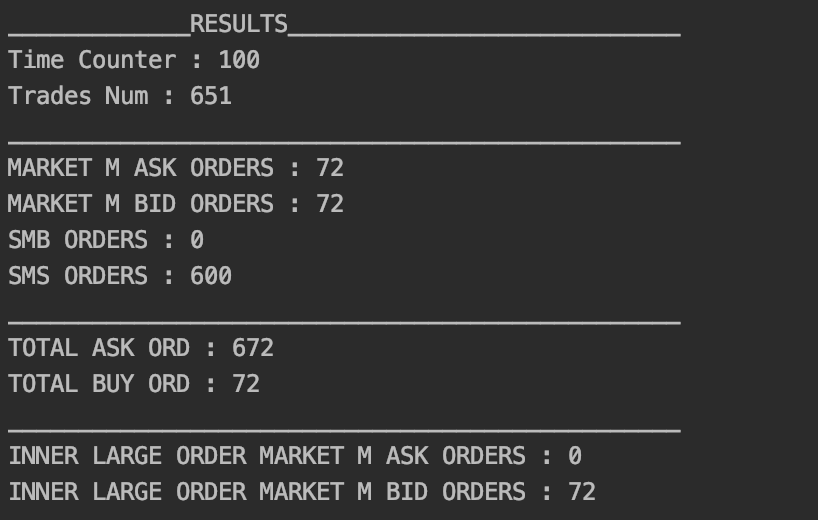
\includegraphics[width=7cm, height=6cm]{Dissertation/images/mcg_indv/SMS.png}
    \caption{Market maker with Simple Seller}
    \label{fig:indv_mm_1}
  \end{subfigure}
  %
  \begin{subfigure}[b]{0.5\textwidth}
    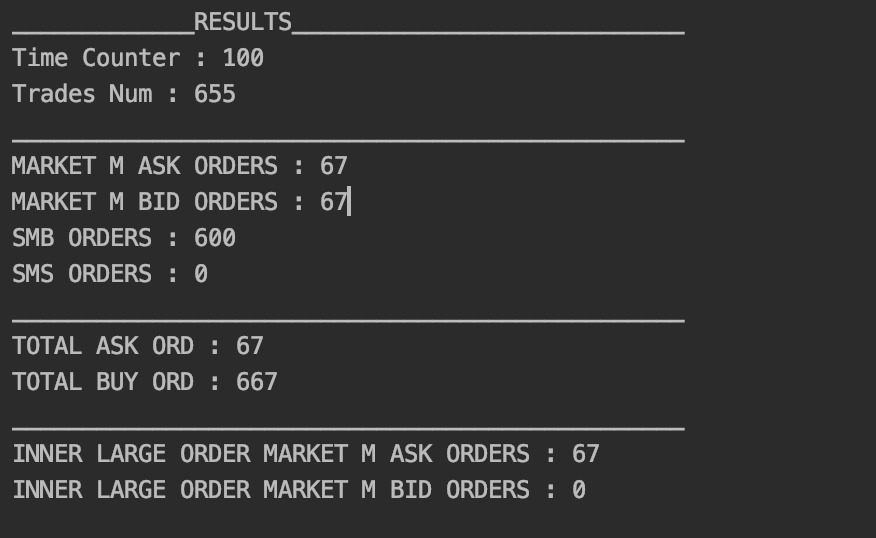
\includegraphics[width= 7cm, height=6cm]{Dissertation/images/mcg_indv/SMB.png}
    \caption{Market maker with Simple Buyer}
    \label{fig:indv_mm_2}
  \end{subfigure}
\caption{Market maker with Simple agent statistics} 
\end{figure}
\FloatBarrier

In Figure \ref{fig:indv_mm_1}, it can be seen that the bid large order of the Market maker is the only one submitted (72 submitted). This is because all of the orders in the Market submitted by the Simple Seller is an ask order. This means that only Condition 1 of Algorithm \ref{algo:market_maker} will be executed.  In addition, the number of total asks and bids submitted by the Market maker is also 72 because in each iteration, the Market maker submits both a bid and an ask order with the bid order at quantity $v^-$. 

Vice versa with Figure \ref{fig:indv_mm_2} where only ask large orders are submitted. This means that only Condition 2 of Algorithm \ref{algo:market_maker} will be executed because there are only bid orders submitted by the Simple Buyer agent.

\section{Liquidity consumer} 
In McG, the Liquidity consumer is also modelled closely to the Oesch 2014 \cite{Oesch} paper. Liquidity consumer represents large financial institution that makes trading decisions based on re-balancing the portfolio. At the start of the day, the agent decides, with equal probability, to sell or buy for the whole day. The Liquidity consumer will trade according to this large order, if empty, will generate a new one. In order to illustrate its behaviour, we adapted the Liquidity trader, only in this test, to draw an initial large order only once in the whole experiment. Note that by submitting market orders, only quantity is specified and not price since the market orders will execute at any price point until the quantity is fulfilled.  
\\
\begin{algorithm}[hbpt!]
\DontPrintSemicolon  
\If{start of the day} {
    \If{$random() > 0.5$} {
    Decides to Buy\;
    }
    \Else{
    Decides to Sell;\
    }
    \EndIf
    Initialize initial large order with volume $h_0 = U(h_{min},h_{max})$\;  
  }
\EndIf

\If{$random() < \delta_{lc}$} {
    \tcc{$\phi_t = $  the volume at the opposite best price at time t}
    \tcc{$h_t = $ is the remaining volume at time t}
    \tcc{Condition 1} 
    \If{$h_t \leq \phi_t$} {
    Submit market order with volume $v_t = h_t$\;
    }
    \tcc{Condition 2}
    \Else{
    Submit market order with volume $v_t = \phi_t$;\
    }
    \EndIf
    $h_t = h_t - v_t$\;  
  }
\EndIf
\caption{{\sc Liquidity consumer reproduced from McG (4.2) \cite{McGroarty} }}
\label{algo:liquidity_consumer}
\end{algorithm}

\begin{table}[h]
\centering
\begin{tabular}{ |m||p{4cm}|} 
\hline
\textbf{Liquidity consumer Parameters}& \textbf{Value} \\
\hline
\hline
$h_{min}$ & 1 \\ 
\hline
$h_{max}$ & 100,000\\ 
\hline
\end{tabular}
\caption{Liquidity consumer parameters taken from \cite{McGroarty} and  \cite{Oesch}} 
\end{table}
\FloatBarrier 

Because the Liquidity consumer only submits a market order, the only test that is viable is to see the quantity the agent has submitted. There are two cases that the quantity of a Liquidity trader will differ. The first case is when the best quantity of the opposite side is more than the remaining quantity and vice versa. The two tests below will demonstrate the agent's behaviour in both cases. Figures \ref{fig:liq_indv_1} and \ref{fig:liq_indv_1} illustrate the quantity of orders submitted in the whole market. The two tests consists of 6 Liquidity consumer and 6 Simple Seller. 

\begin{figure}[h]
  \begin{subfigure}[b]{0.5\textwidth}
    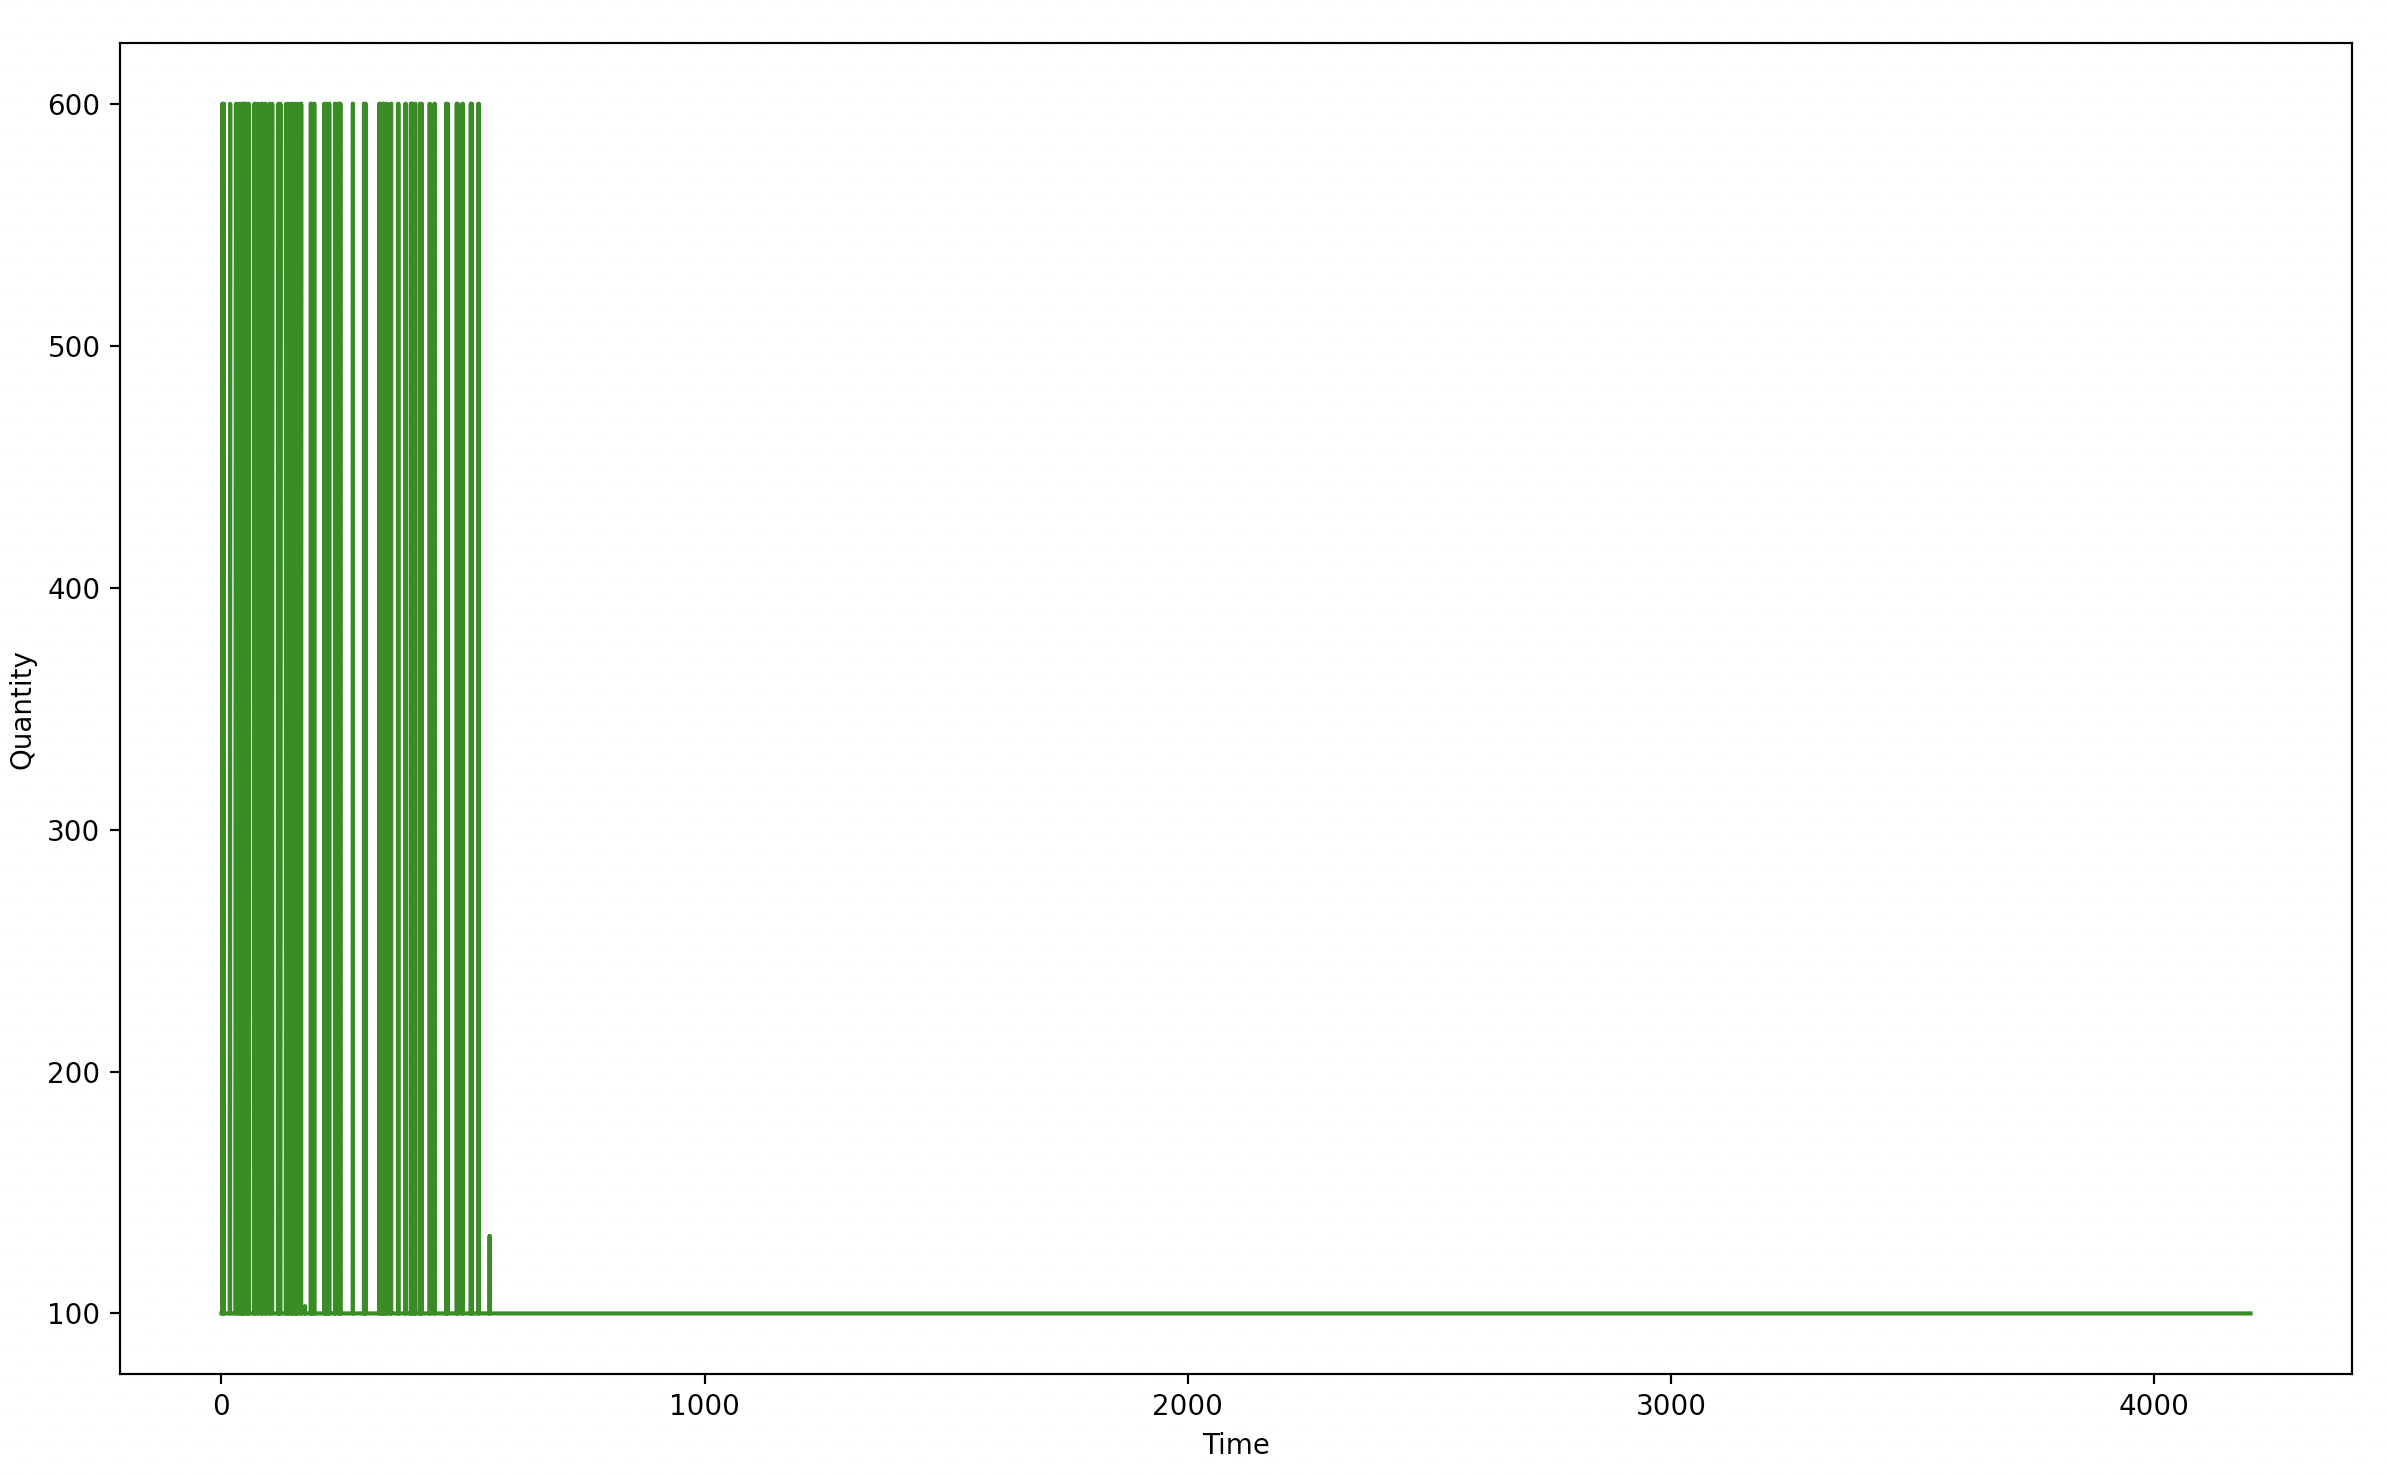
\includegraphics[width=7cm, height=6cm]{Dissertation/images/mcg_indv/LIQ/100.png}
    \caption{Case A : Simple seller quantity of 100 in 4200 McG action steps}
    \label{fig:liq_indv_1}
  \end{subfigure}
  %
  \begin{subfigure}[b]{0.5\textwidth}
    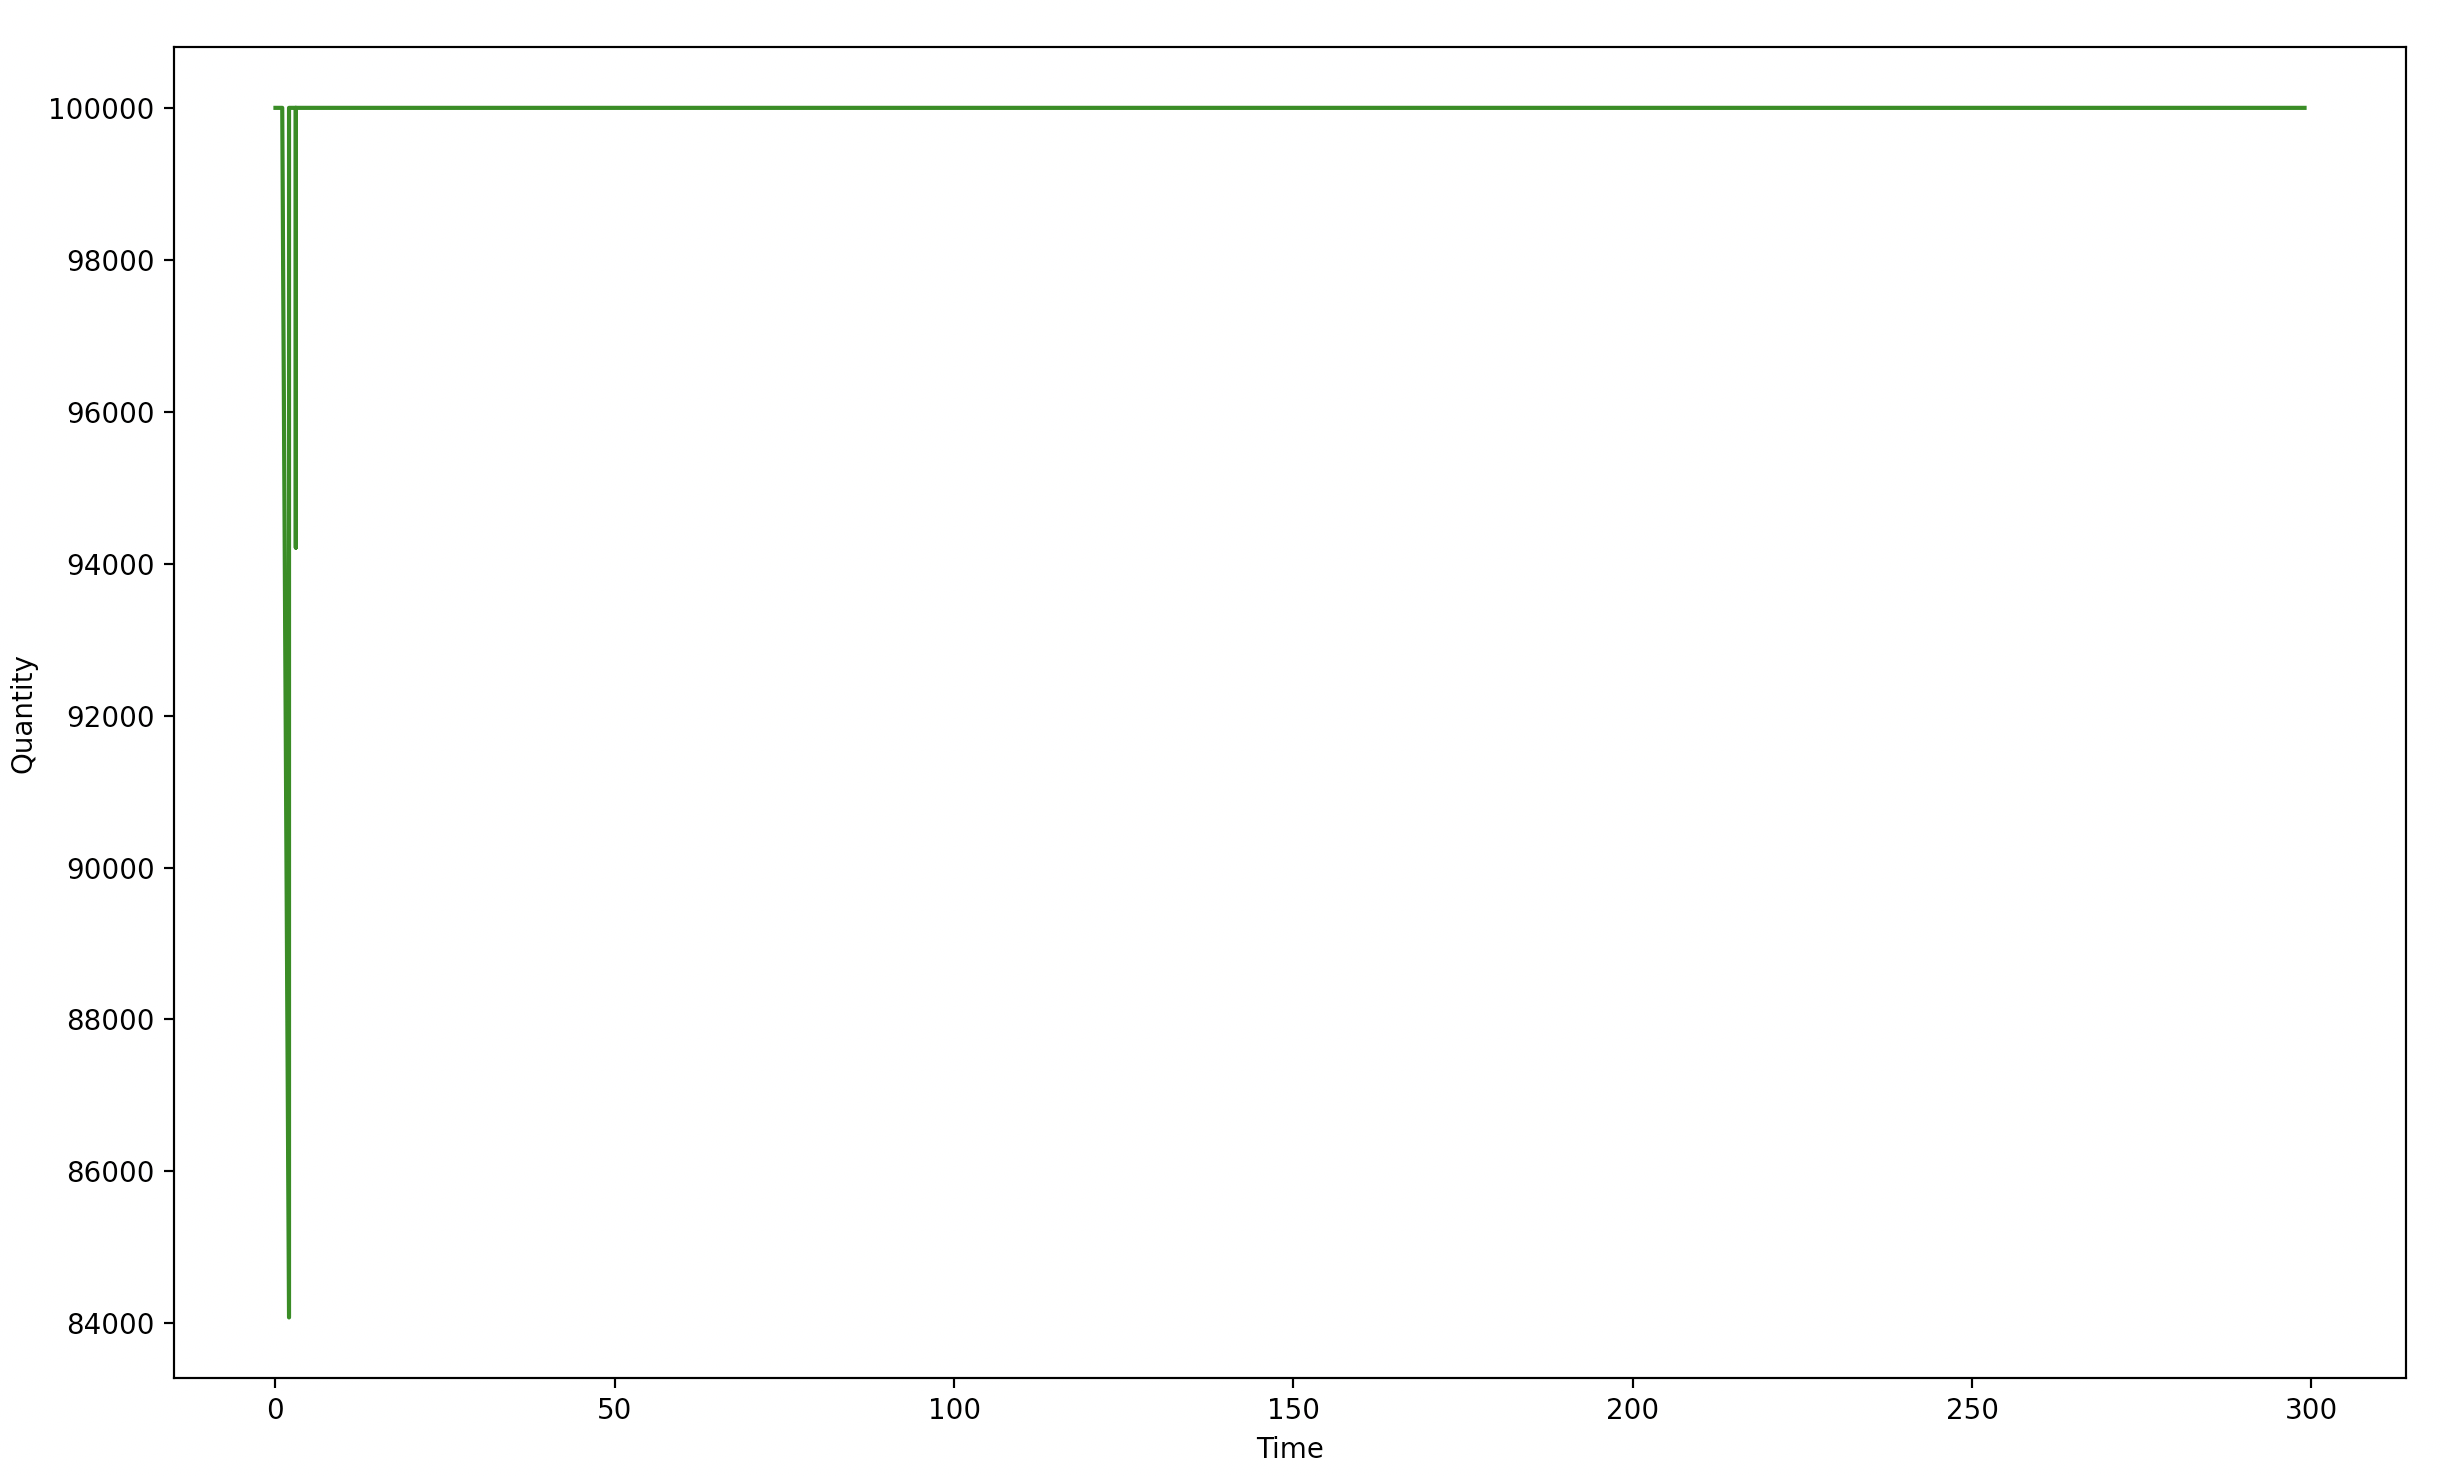
\includegraphics[width= 7cm, height=6cm]{Dissertation/images/mcg_indv/LIQ/san.png}
    \caption{Case B : Simple seller quantity of 100,000 in 300 McG action steps}
    \label{fig:liq_indv_2}
  \end{subfigure}
\caption{Quantity of each order submitted : Liquidity consumer with Simple Seller submitting different quantity of orders in 4200 McG action steps} 
\end{figure}
\FloatBarrier

\textbf{Case A:} The first case in Figure \ref{fig:liq_indv_1} is when the Simple sellers are only submitting orders at $price = 100$ and $quantity = 100$. It can be seen that in the initial period of the market, the orders submitted is 600. Theses are all orders submitted by the Liquidity consumer agents because their initially drawn large order is much higher than what is available in the market. The number is 600 because there are 6 Simple sellers who are all submitting orders of 100 quantity. Hence, they submit what is the maximum quantity at the best price of the opposite side of the book which is directly in Condition 2 on Line 8 in Algorithm \ref{algo:liquidity_consumer}. 

\textbf{Case B:} The second case in Figure \ref{fig:liq_indv_2} is when Simple sellers are submitting at $price = 100$ and $quantity = 100,000$. This means that traders who have been assigned with "Bid" day task will submit their initial large order and then stop after submitting one order because they are able to submit their whole large order since the orders at the opposite side of the book is much larger than their initial large order. This is because the agents' large is drawn uniformly from 1 to 100,000 while the Simple agents are submitting at only 100,000. The smaller values than 100,000 in the initial period of the market is from Liquidity consumer submitting their whole initially drawn large orders. This is Condition 1 on line 10 of the Algorithm \ref{algo:liquidity_consumer}. The rest of the orders seen in the market at 100,000 quantity is from only Simple Sellers.

The case where there are only Simple Buyers is omitted because the results would be similar except the Liquidity consumer would only submit ask orders because there are only bid orders in the LOB. 


\section{Momentum trader}
The momentum trader is one of two the high frequency trader who submit according to the market current price movement. A momentum trader trades depending on the rate of change in the price movement. The trader will submit a bid order if the price has recently been rising and an ask order otherwise. The calculation of Rate of Change (ROC) is given by: 
\begin{equation}
    roc_t = \frac{p_t - p_{t-n_r}}{p_{t-n_r}}
\end{equation}
\newline where $p_t$ = price at time t, $n_r$ = the period where the agent will calculate the ROC 

\newline When $roc_t$ is greater than some threshold $\kappa$, the agent submits a bid order with the volume described as:
\begin{equation}
     v_t = \abs{roc_t} * W_{a,t} 
\end{equation}
\newline where $roc_t$ = ROC at time t, $W_{a,t}$ = the wealth of the agent at time $t$. 

\begin{algorithm}[H]
\DontPrintSemicolon 
\If{$random() < \delta_{mt}$} {
    \tcc{Condition 1} 
    \If{$roc_t \ge \kappa$} {
    Submit market buy order with volume $v_t = \abs{roc_t} * W_{a,t}$\;
    }
    \tcc{Condition 2} 
    \uElseIf{$roc_t \leq -\kappa$}{
    Submit market sell order with volume $v_t = \abs{roc_t} * W_{a,t}$;\
    }
    \EndIf
  }
\EndIf
Update ROC $roc_t = \frac{p_t - p_{t-n_r}}{p_{t-n_r}}$\;  
\caption{{\sc Momentum trader reproduced from McG (4.3) \cite{McGroarty} } }
\label{algo:momentum}
\end{algorithm}

\begin{table}[h]
\centering
\begin{tabular}{ |m||p{4cm}|} 
\hline
\textbf{Momentum trader Parameters}& \textbf{Value} \\
\hline
\hline
$n_r$ & 5 \\ 
\hline
$\kappa$ & 0.001\\ 
\hline
$V_{mt}$ & 500,000 (100,000 in the test) \\ 
\hline
\end{tabular}
\caption{Momentum trader parameters taken from \cite{McGroarty}} 
\end{table}
\FloatBarrier 

\subsection{Momentum trader's Wealth}
One of the important variable in the Momentum trader's trading strategy is its wealth. The agent will submit the quantity of an order based on its wealth given by equation : $v_t = \abs{roc_t} * W_{a,t}$. The concept of Wealth $W_{a,t}$ is different in this BSE implementation due to the fact that the agent can submit either a bid or an ask in any order. In reality, a trader can submit an ask then buy back the stocks at a later date. Similarly, one can buy a quantity of stock and sell it back at a later date. Because the Momentum trader does not have that constraint, there must be some abstraction in calculation of wealth. 

The approach taken in this project is as follow: The wealth will be separated into two types : Ask balance and Bid balance. 

\begin{itemize}
  \item \textbf{Ask Balance} : The initial price is 0. This is due to the fact that if someone sells a product, their wealth will increase. After the agent's market order is fulfilled, their ask balance will increase by $quantity * price_{transaction}$. This idea is abstracted from the fact that the agent can sell something it does not have. The ask balance will be capped at $V_{mt}$. 
  \item \textbf{Bid Balance} : The initial price is $V_{mt}$. This is due to the fact that if someone buys a product, their wealth will decrease. After the agent's market order is fulfilled, their bid balance will decrease by $quantity * price_{transaction}$.
\end{itemize}

The wealth $W_{a,t}$ of the agent is then calculated by Ask balance + Bid balance. 

\subsection{Momentum trader Test} 
Similar to Liquidity consumer, the Momentum trader submits only a market order. Hence, in the following experiment, only the quantity and the type of order will be investigated.  

The experiment will consists of two types of price arrangement : increasing and decreasing. This is to investigate whether the momentum trader will respond correctly to the momentum in the price. In order to evaluate the current Momentum trader algorithm, the following test will be conducted. The Simple Seller and Buyer will be modified such that:
\begin{itemize}
  \item It will include a probability of submitting at 0.25 to ensure that the orders don't always match and there is limit orders left in the Limit Order book. 
  \item The Simple agents will submit with quantity drawn uniformly from between 100 and 1000 to ensure that the Limit Order Book is not empty
  \item The agents will submit either a decreasing or increasing price in each iteration. For example, if it is decreasing, the initial price will be 1000 and decremented by 1 in each McG action step. This ensures that the mid price will be a downward slope and the momentum of the market is in the downward slide. 
\end{itemize}

The experiment will run in 1000 McG action step. The market consists of 6 Simple Buyers, 6 Simple Sellers and 6 Momentum trader. The results are illustrated below: 

\begin{figure}[h]
  \begin{subfigure}[b]{0.5\textwidth}
    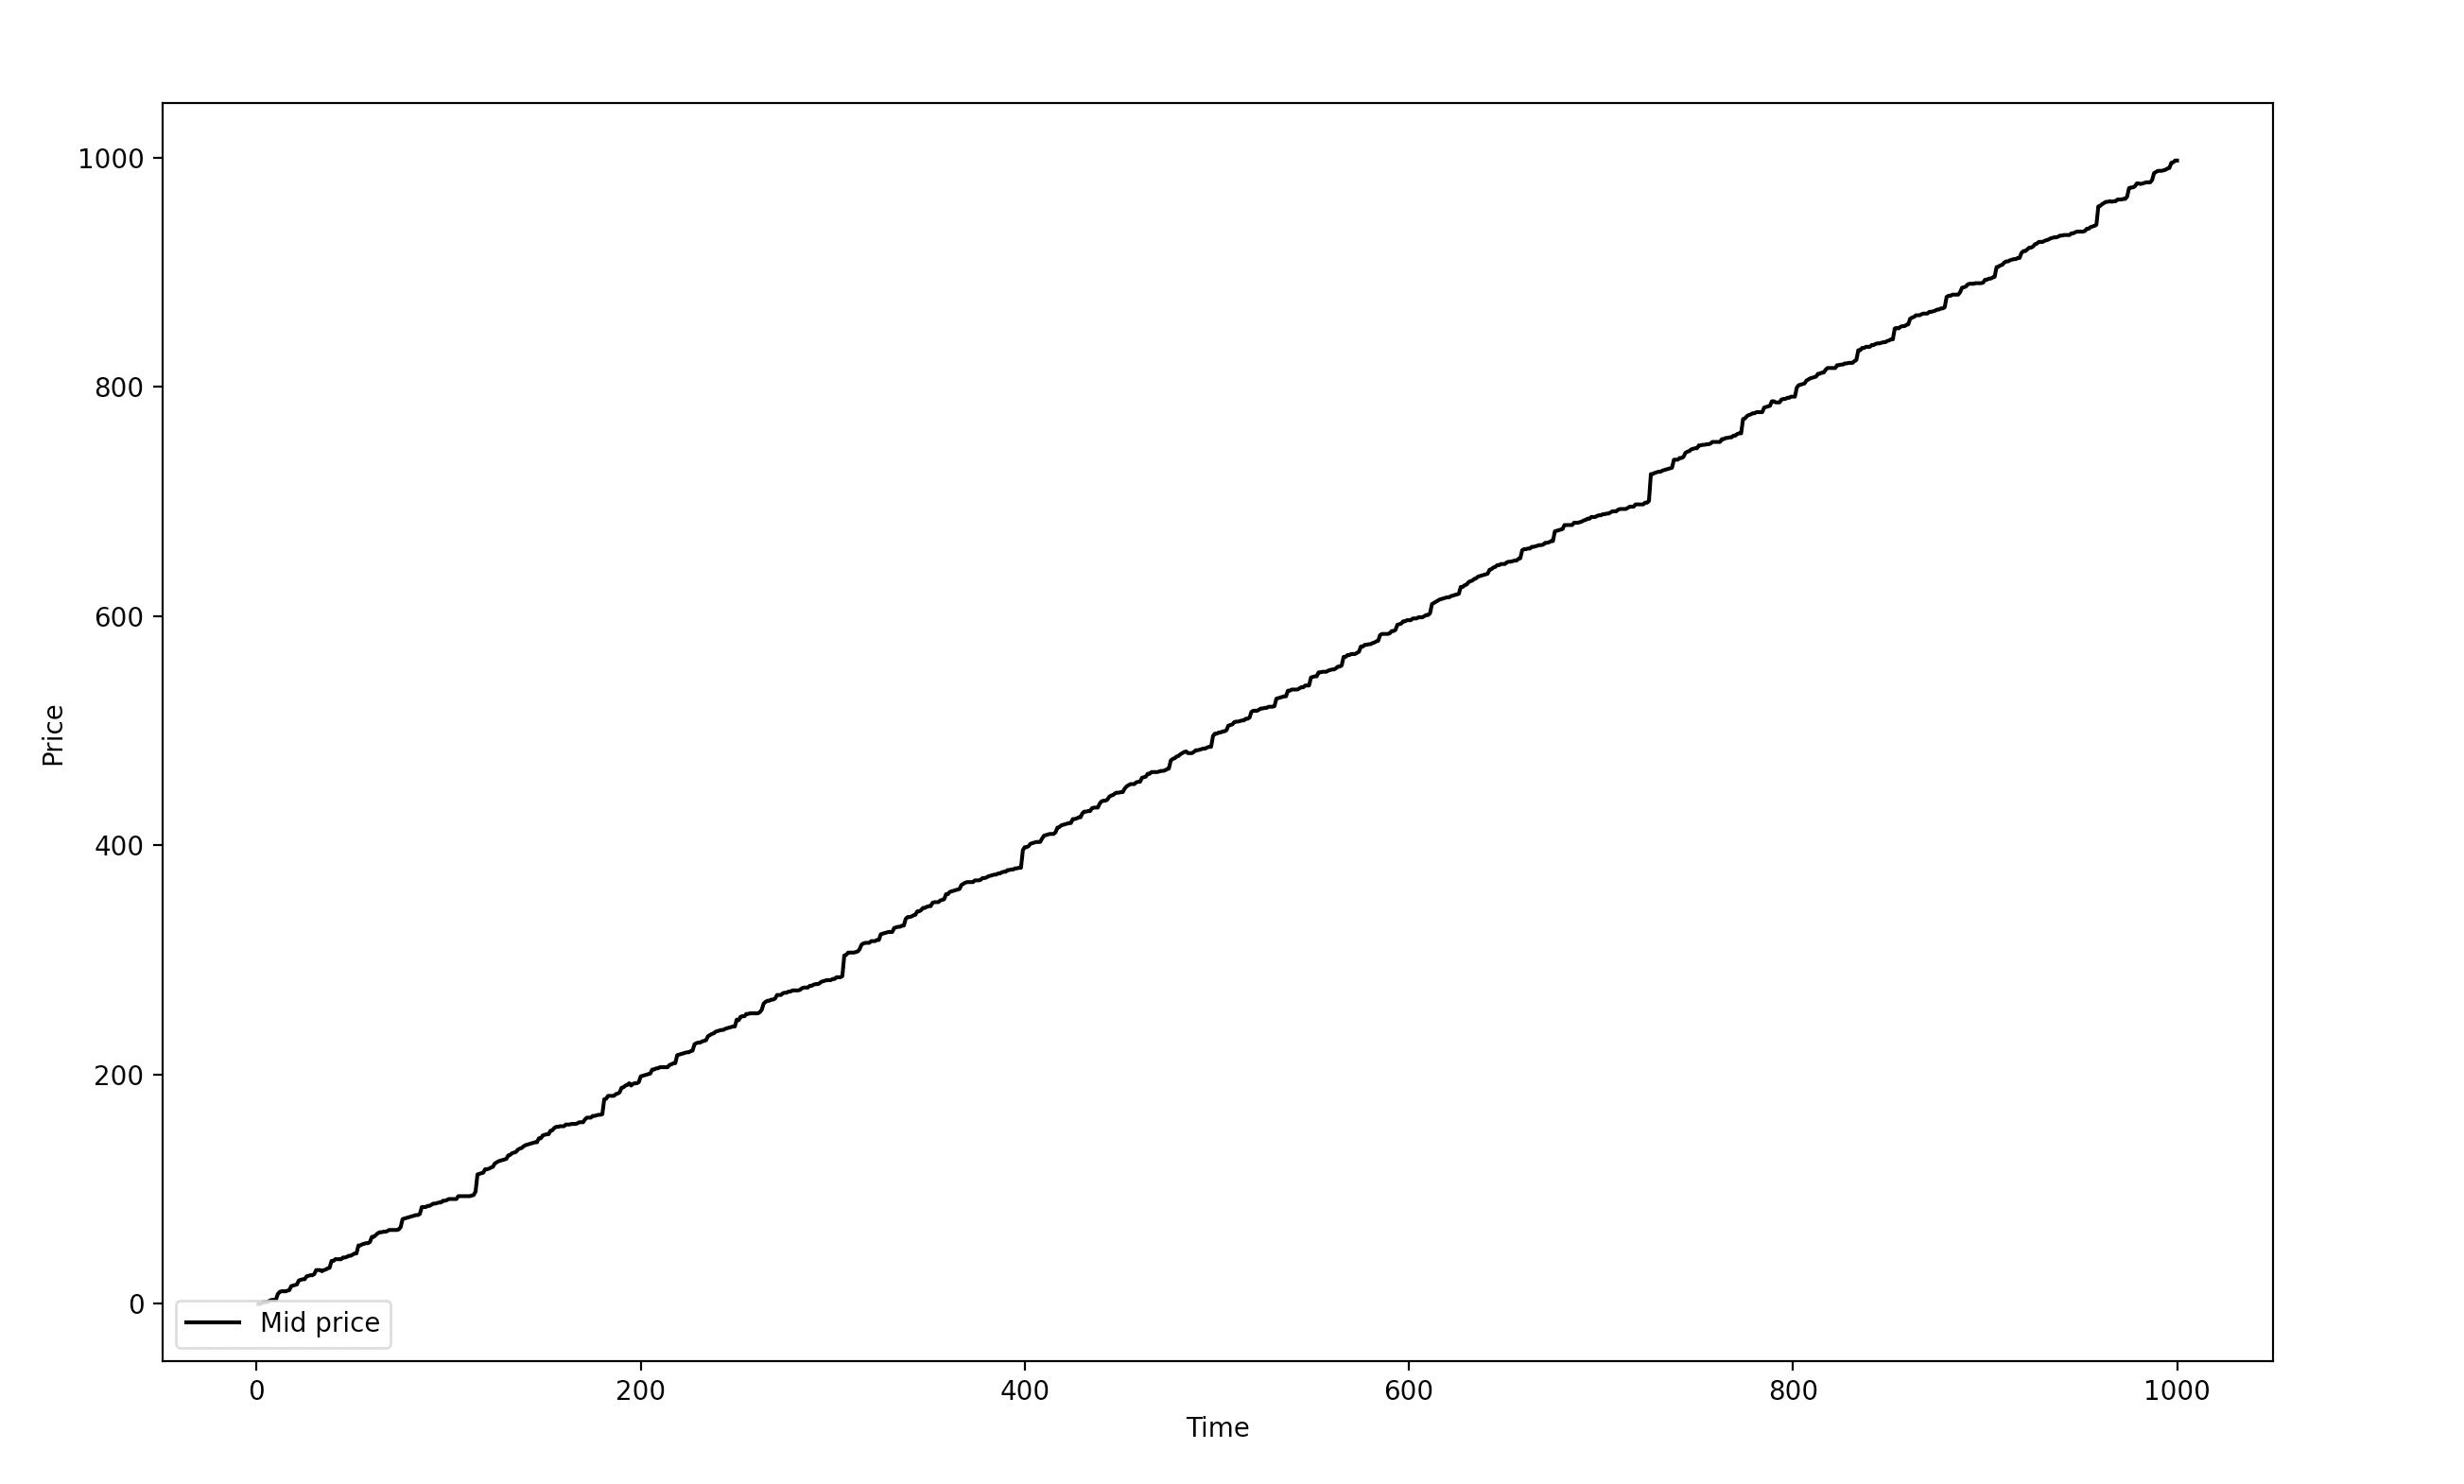
\includegraphics[width=7cm, height=6cm]{Dissertation/images/mcg_indv/MMT/incr.png}
    \caption{Mid Price}
    \label{fig:mmt_inc_midprice}
  \end{subfigure}
  %
  \begin{subfigure}[b]{0.5\textwidth}
    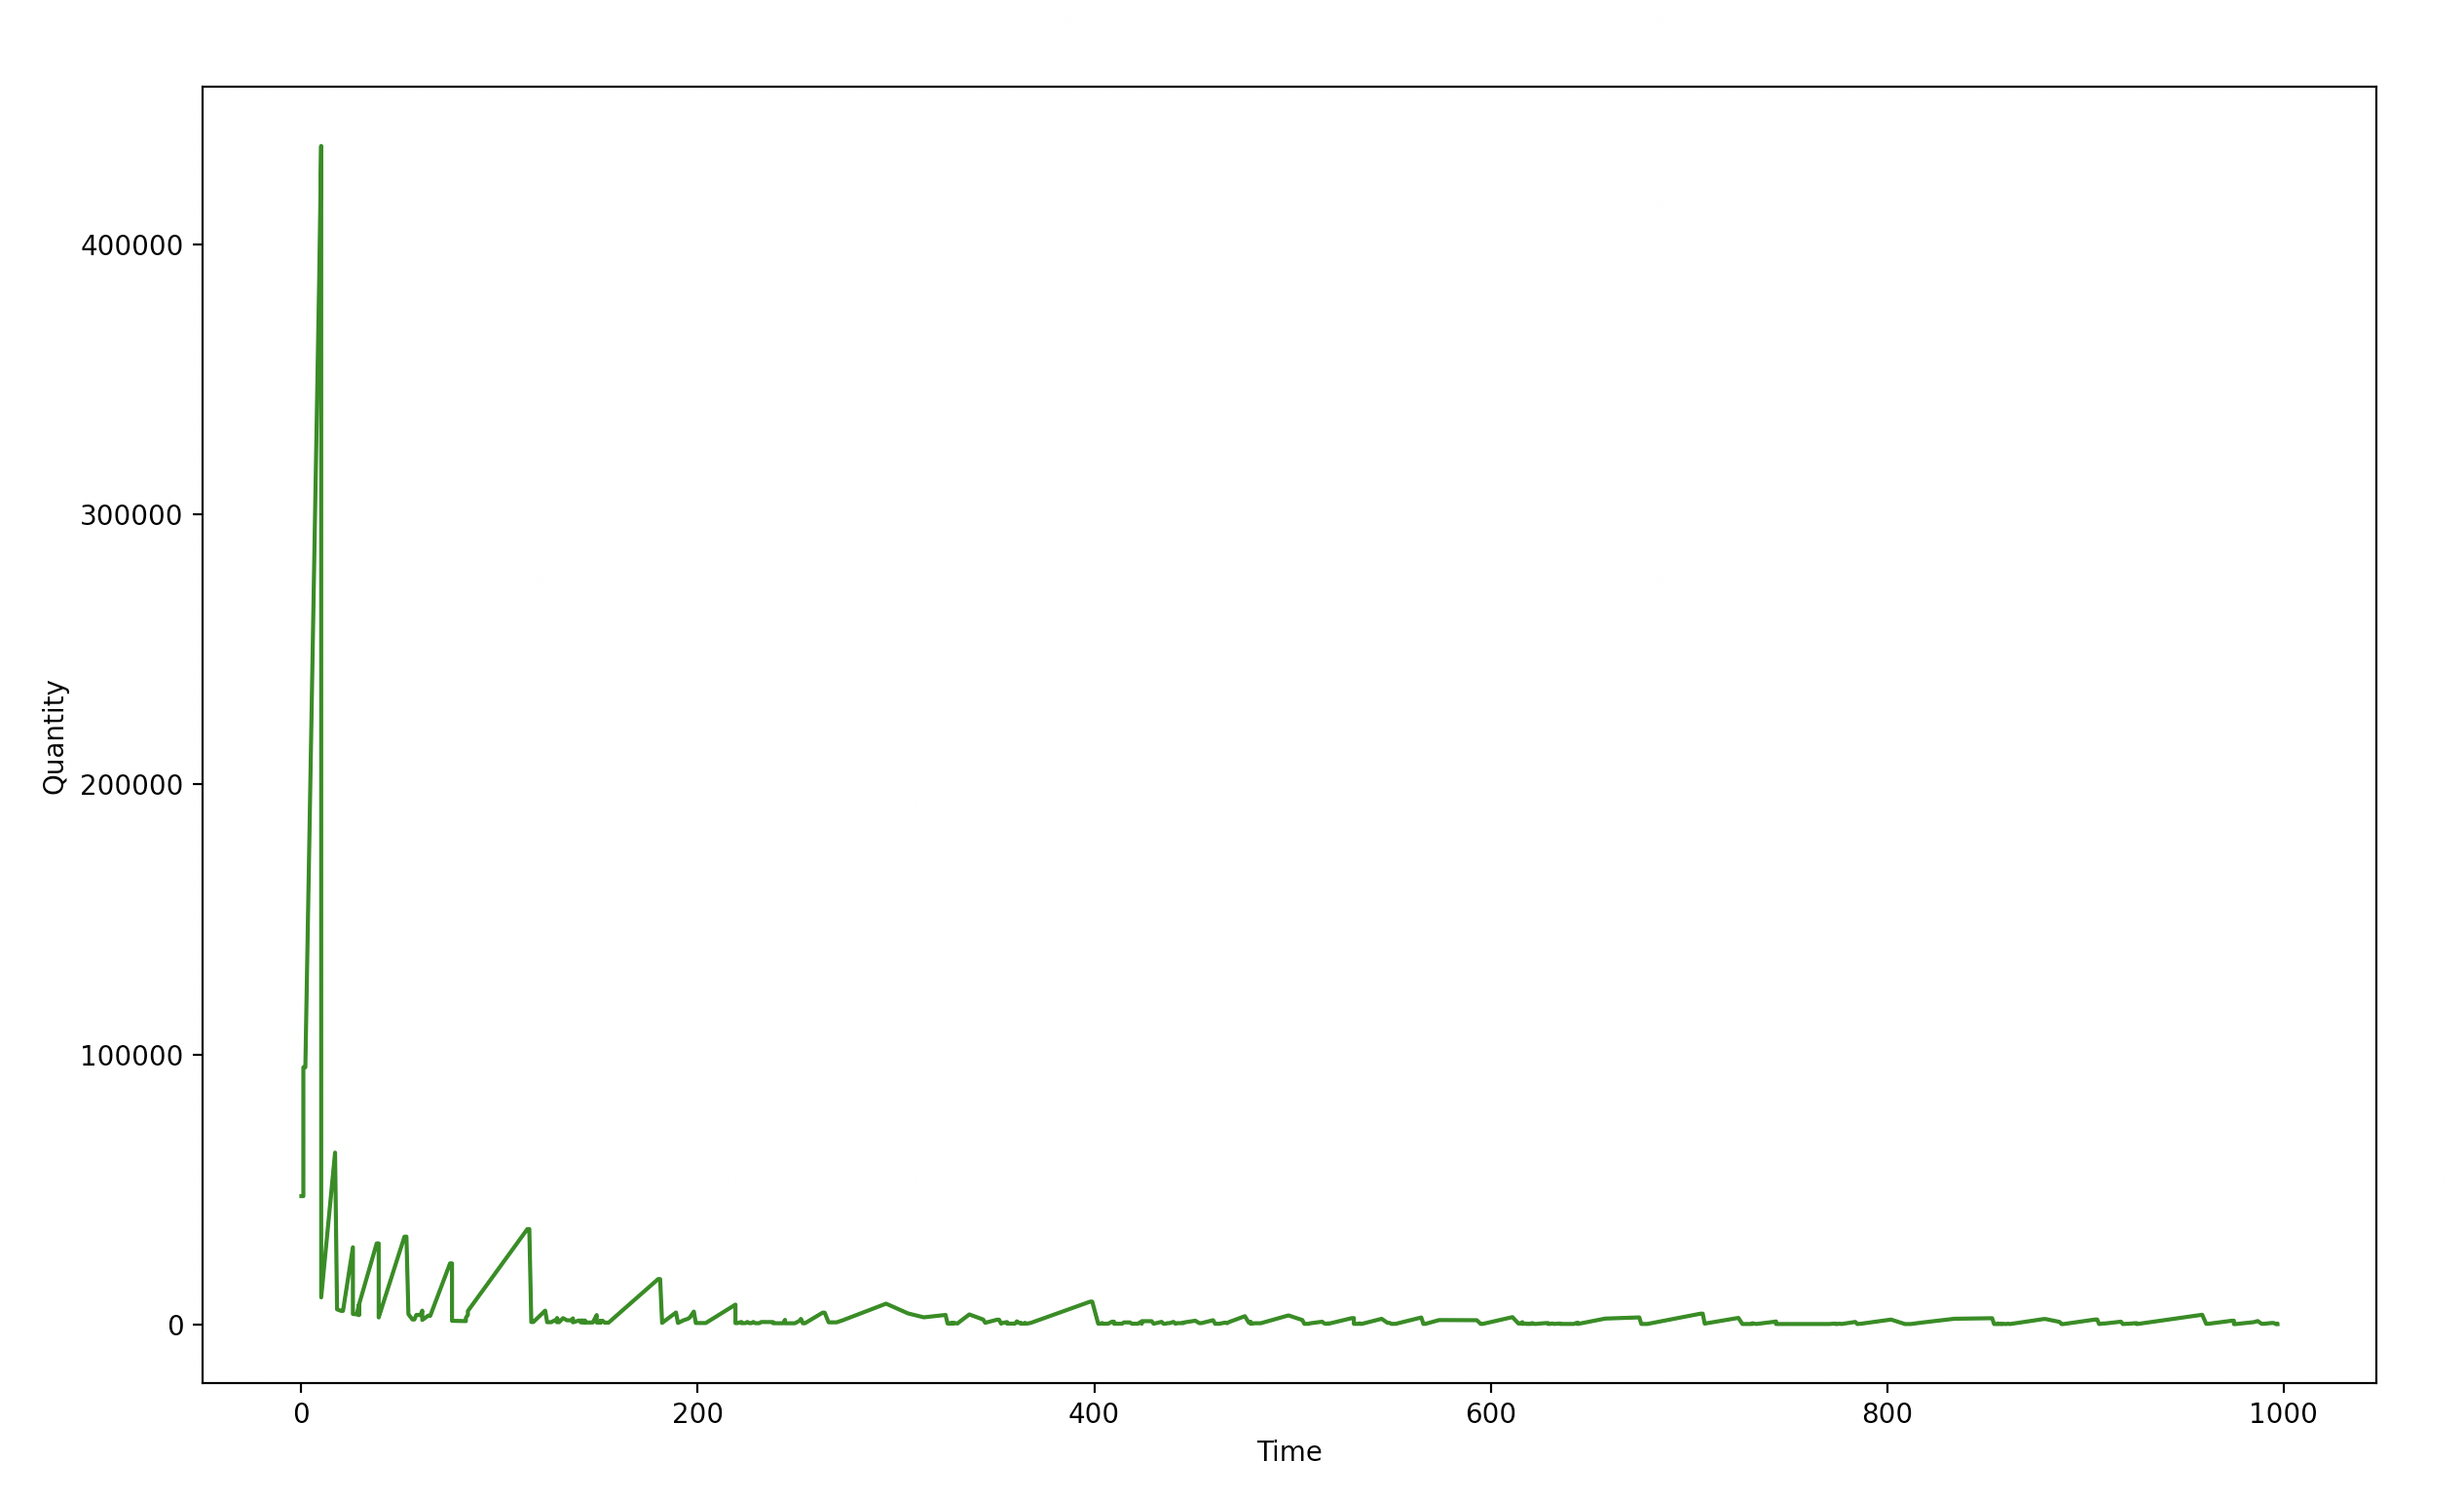
\includegraphics[width= 7cm, height=6cm]{Dissertation/images/mcg_indv/MMT/incr_qty.png}
    \caption{Quantity submitted by Momentum trader both Bid and Ask}
    \label{fig:mmt_inc_qty}
  \end{subfigure}
\caption{Momentum trader increasing price experiment} 
\end{figure}


\begin{figure}[h]
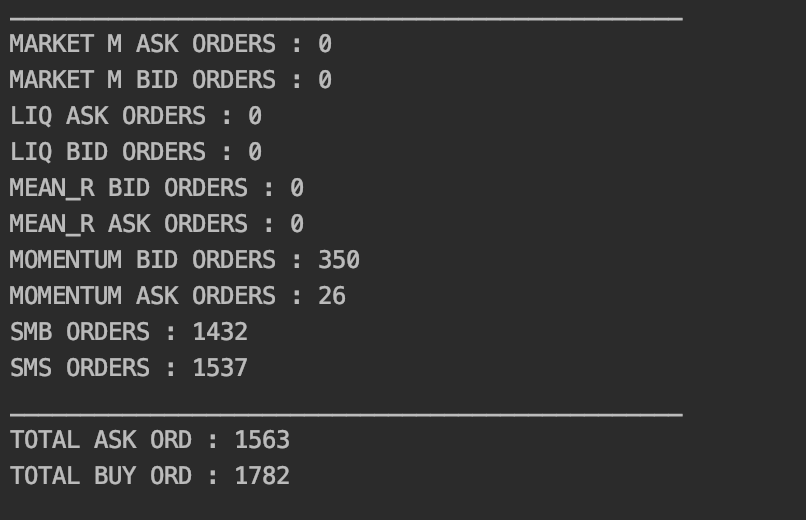
\includegraphics[ height=8cm]{Dissertation/images/mcg_indv/MMT/incr_stat.png}
\caption{Momentum trader increasing price experiment statistics} 
\label{fig:mmt_inc_stats}
\end{figure} 
\FloatBarrier

Figures \ref{fig:mmt_inc_stats}, \ref{fig:mmt_inc_qty} and \ref{fig:mmt_inc_midprice} illustrate the increasing test results of the market. Figure \ref{fig:mmt_inc_midprice} illustrates the mid price which increases over the 1000 time period. In Figure \ref{fig:mmt_inc_qty}, The quantity submitted by Momentum traders will quickly decrease because of the reduction in its wealth. This is because the agents are only buying because the momentum is going in upwards direction.This is directly from the line 2 or the first condition of the Algorithm \ref{algo:momentum}. 

In most cases, the price submitted from the trader at time t will be more than $t-n_r$. For example, if $p_t = 80$ then $p_{t - n_r} = 70$. This means that the $roc_t$ will be 0.114. According to the first condition of the Algorithm 4.3, $0.114 \ge 0.001$, which is true, the agent will submit a buy order, leading to the decreasing wealth described above.  

\begin{figure}[h]
  \begin{subfigure}[b]{0.5\textwidth}
    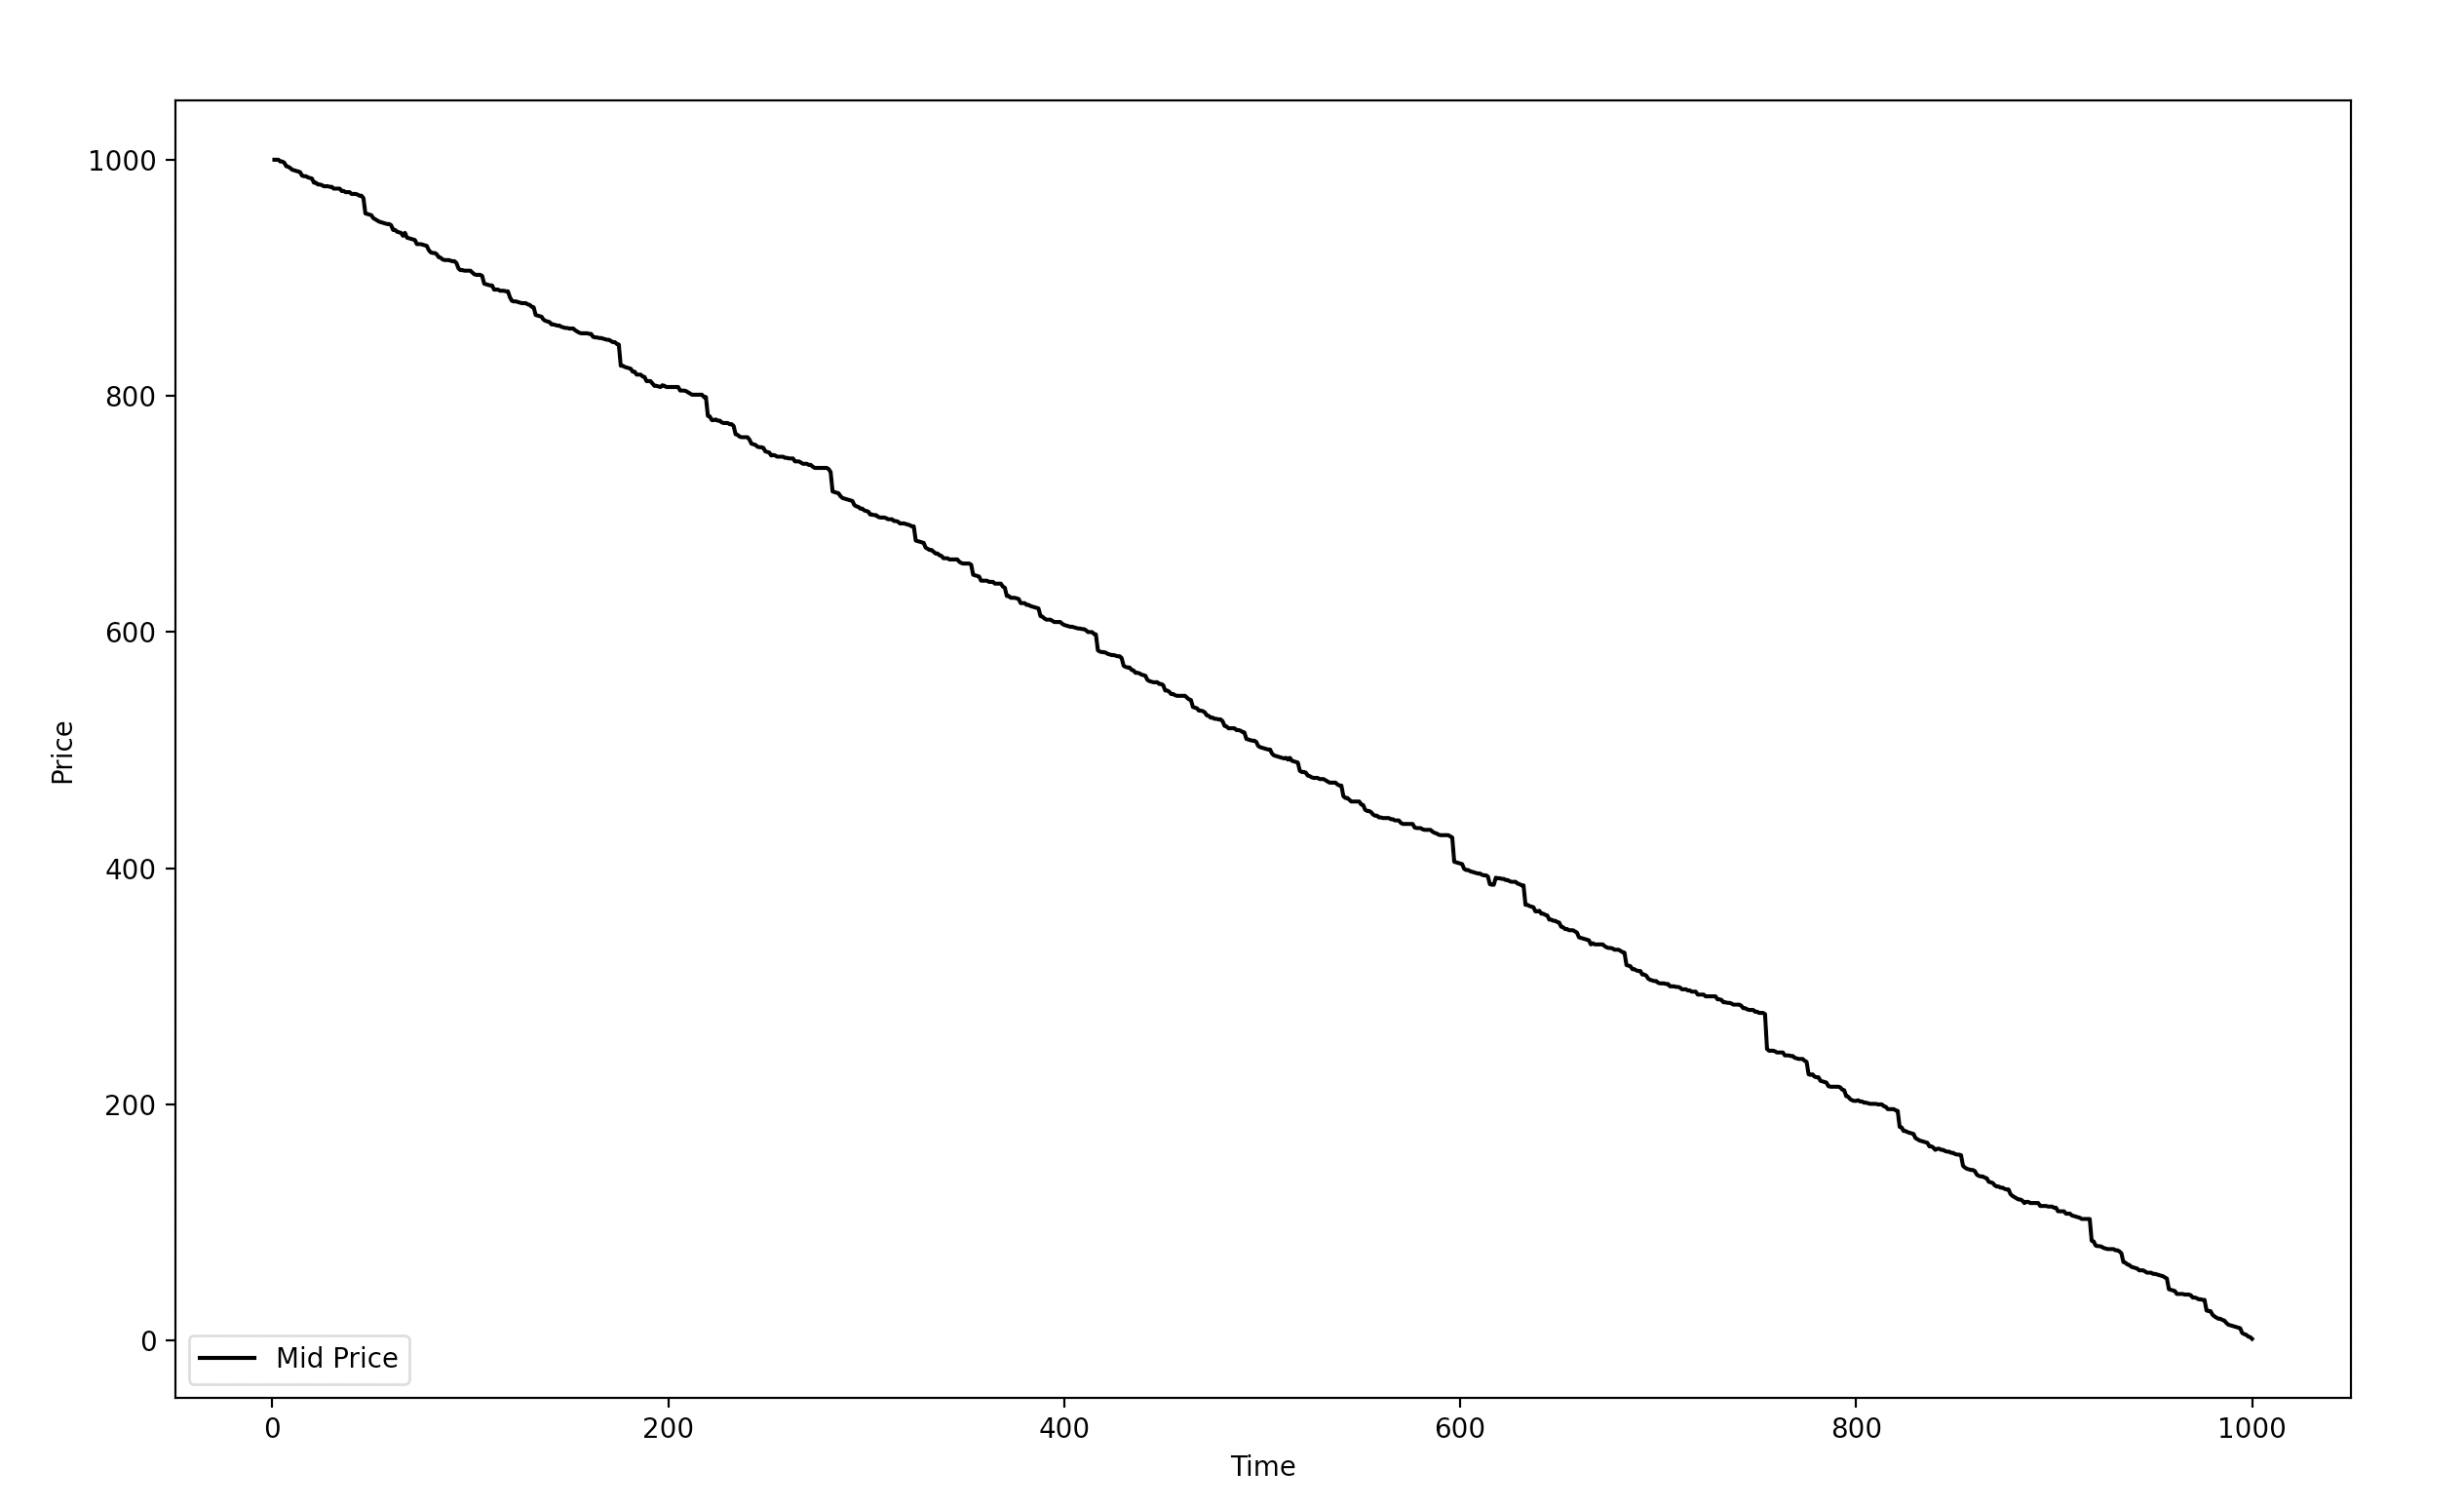
\includegraphics[width=7cm, height=6cm]{Dissertation/images/mcg_indv/MMT/dec_price.png}
    \caption{Mid Price}
    \label{fig:mmt_dec_midprice}
  \end{subfigure}
  %
  \begin{subfigure}[b]{0.5\textwidth}
    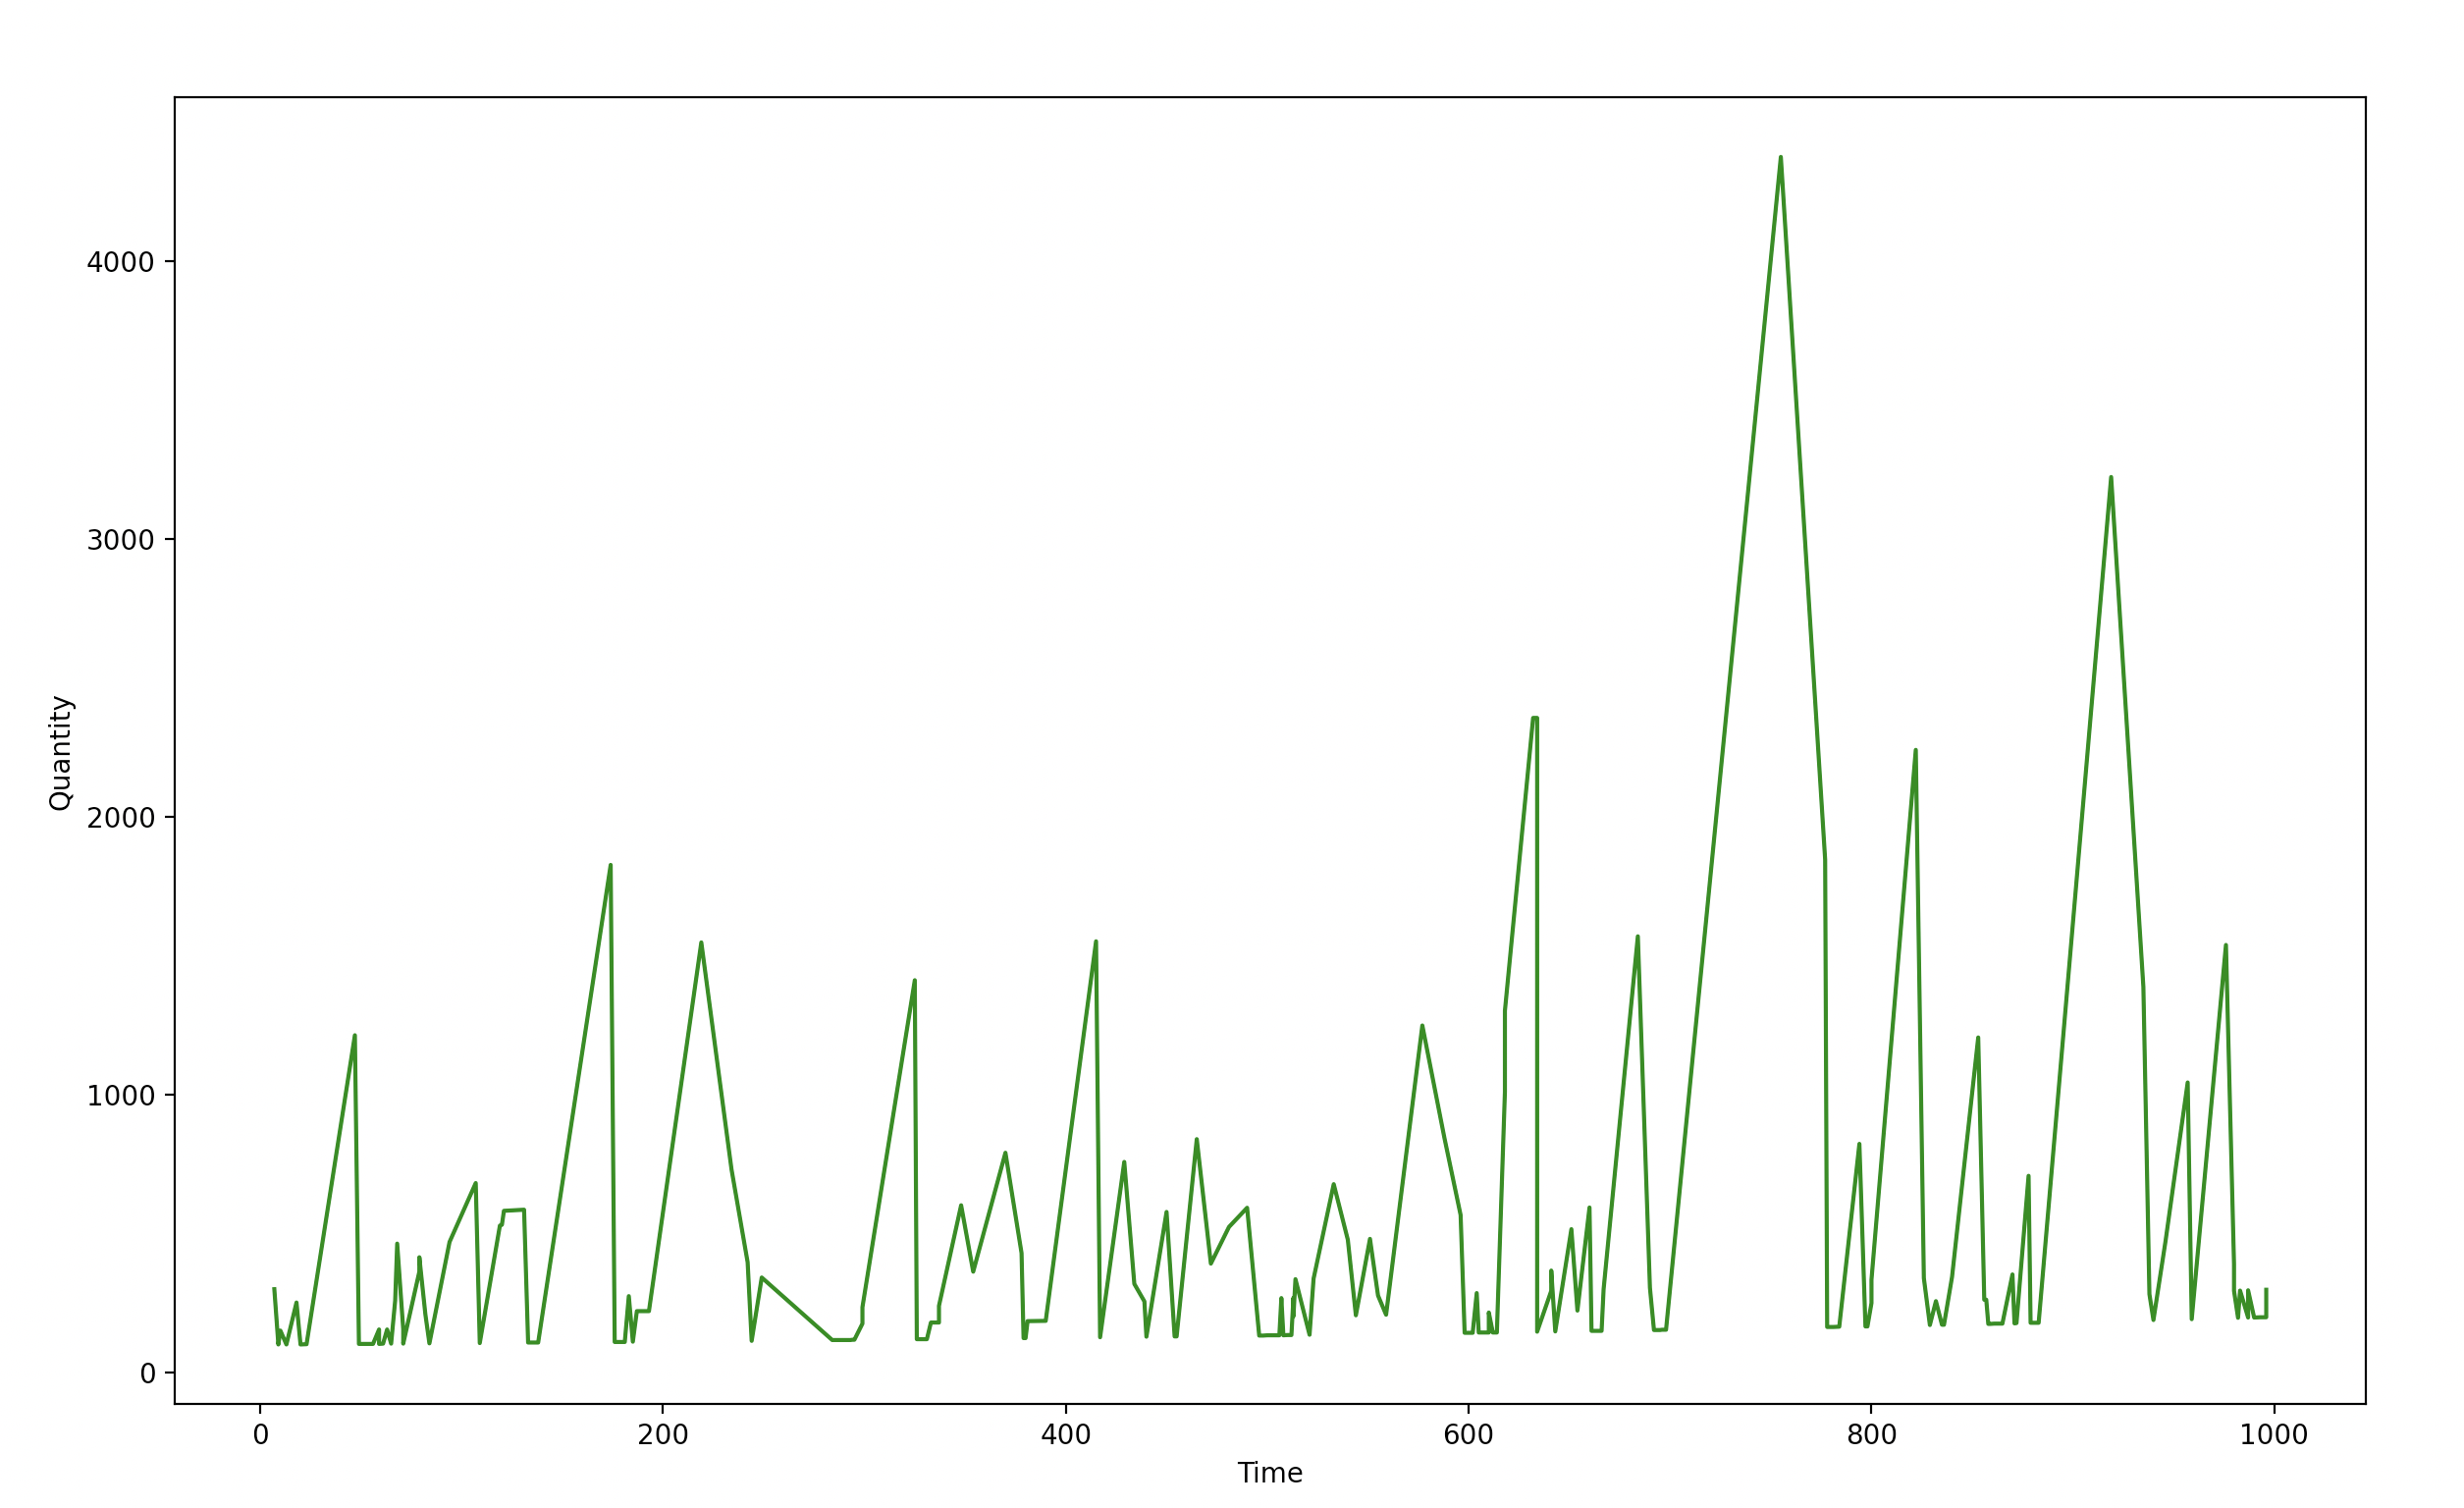
\includegraphics[width= 7cm, height=6cm]{Dissertation/images/mcg_indv/MMT/dec_qty.png}
    \caption{Quantity submitted by Momentum trader both Bid and Ask}
    \label{fig:mmt_dec_qty}
  \end{subfigure}
\caption{Momentum trader decreasing price experiment} 
\end{figure}


\begin{figure}[h]
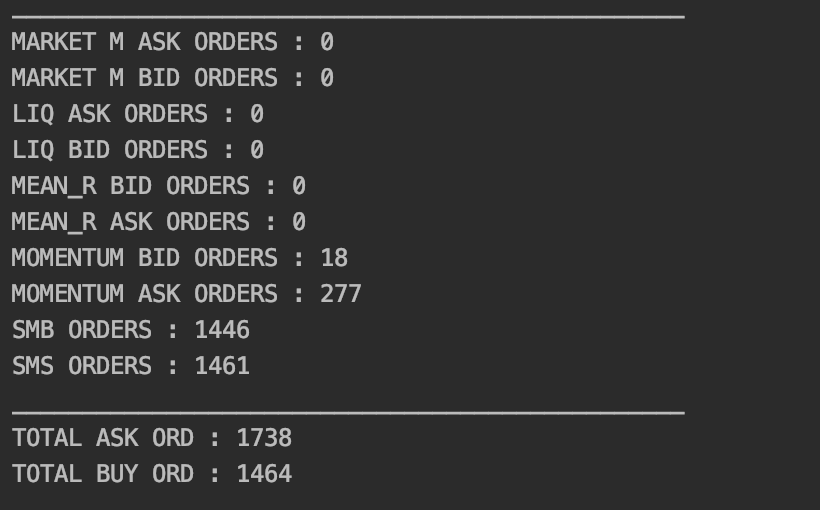
\includegraphics[ height=8cm]{Dissertation/images/mcg_indv/MMT/dec_stat.png}
\caption{Momentum trader decreasing price experiment statistics} 
\label{fig:mmt_dec_stats}
\end{figure} 
\FloatBarrier

Figures \ref{fig:mmt_dec_midprice}, \ref{fig:mmt_dec_qty}  and \ref{fig:mmt_dec_stats} illustrate the decreasing test results of the market. Figure \ref{fig:mmt_dec_midprice} illustrates the mid price which decreases over the 1000 time period. The quantity over time in this experiment is increasing since the agents are submitting only ask orders, hence their wealth is increasing over time. This is directly from line 4 or the second condition of the Algorithm \ref{algo:momentum} where we can see the Momentum of the market going downwards from Figure \ref{fig:mmt_dec_qty}. The majority of the order submitted in Figure \ref{fig:mmt_dec_stats} will be asks orders because the market is gaining an downward momentum. 

In most cases, the price submitted from the trader at time t will be less than $t-n_r$. For example, if $p_t = 70$ then $p_{t - n_r} = 80$. This means that the $roc_t$ will be $-0.125$. According to the second condition of Algorithm \ref{algo:momentum}, $-0.125 \leq -0.001$, which is true, the agent will submit a sell order, leading to the increasing wealth described above.

To clarify, most of the orders are either ask or bid but in some cases they also submit the opposite type of order because of the mid-price. In some cases, the mid price can be [70, 69, 68 ,74, 66] because the Simple Sellers and Buyers have a probability of submitting an order at 0.25, hence the best price orders may not always match. When the Momentum agent evaluates the mid-price pattern, it does not see the decreasing trend but rather the difference between 70 and 74 since they are $n_r = 4$ apart, which is an increasing trend. Hence, it submits a bid instead of an ask. This rarely happens in the Oesch and McG experiments in the Chapter 5 and Chapter 6 since there are more orders in the market and the mid price often moves in a single direction. 

\section{Mean reversion trader}
The Mean reversion trader is intended to represent one type of the two high frequency traders who believes that the price of the market will always revert back to the rolling-average line.  This means that they submit a bid order when the current price is below the average and an ask order when it is above. The exponential moving average is given by: 
\begin{equation}
    ema_t = ema_{(t-1)} - \alpha(p_t - ema_{(t-1)})
\end{equation}
where $p_t$ is price at time $t$ and $\alpha$ is a discount coefficient that adjust the recency bias. If the current price $p_t$ is $k$ standard deviation above $ema_t$, the agent submits a sell order and a buy order if it is $k$ standard deviation below $ema_t$. The volume is denote by $v_{mr}$.The mean reversion behaviour is better illustrated with a simpler unit test with no other agents in the market.

\begin{algorithm}[H]
\DontPrintSemicolon 
\If{$random() < \delta_{mr}$} {
    \If{$p_t - ema_t \ge k\sigma_t$} {
    Submit sell just inside best price with $v_t = v_{mr}$\;
    }
    \uElseIf{$ema_t - p_t \ge k\sigma_t$}{
    Submit buy just inside best price with $v_t = v_{mr}$\;
    }
    \EndIf
  }
\EndIf
Update $ema_t$ = $ema_{(t-1)} - \alpha(p_t - ema_{(t-1)})$
\caption{{\sc Mean reversion trader reproduced from McG (4.4) \cite{McGroarty}} }
\label{algo:max}
\end{algorithm}

\begin{table}[h]
\centering
\begin{tabular}{ |m||p{4cm}|} 
\hline
\textbf{Mean Reversion consumer Parameters}& \textbf{Value} \\
\hline
\hline
$v_{mr}$ & 1 \\ 
\hline
$\alpha$ & 0.94\\ 
\hline
$k$ & 1 \\ 
\hline
$w_{mr}$ & 50 (10 in the experiment)\\ 
\hline
\end{tabular}
\caption{Mean Reversion consumer parameters taken from \cite{McGroarty}}  
\end{table}
\FloatBarrier

In order to evaluate the current Mean Reversion algorithm, the following test will be conducted. The Simple Seller and Buyer will be modified such that:
\begin{itemize}
  \item It will include a probability of submitting at 0.25 to ensure that the orders don't always match and there is limit orders left in the Limit Order book. 
  \item The agents will submit with quantity drawn uniformly from between 100 and 1000 to ensure that the Limit Order Book is not empty
  \item The agents will submit a random price drawn uniformly between 98 to 102. This is to mimic the price range that will be seen in the real McG experiment. 
\end{itemize}

The following experiment will run for 50 McG time period. The market consists of 1 Mean Reversion trader, 6 Simple Buyer and 6 Simple Seller. The graph represents the behaviour of a single agent in detail. The results are illustrated below. 

\begin{figure}[h]
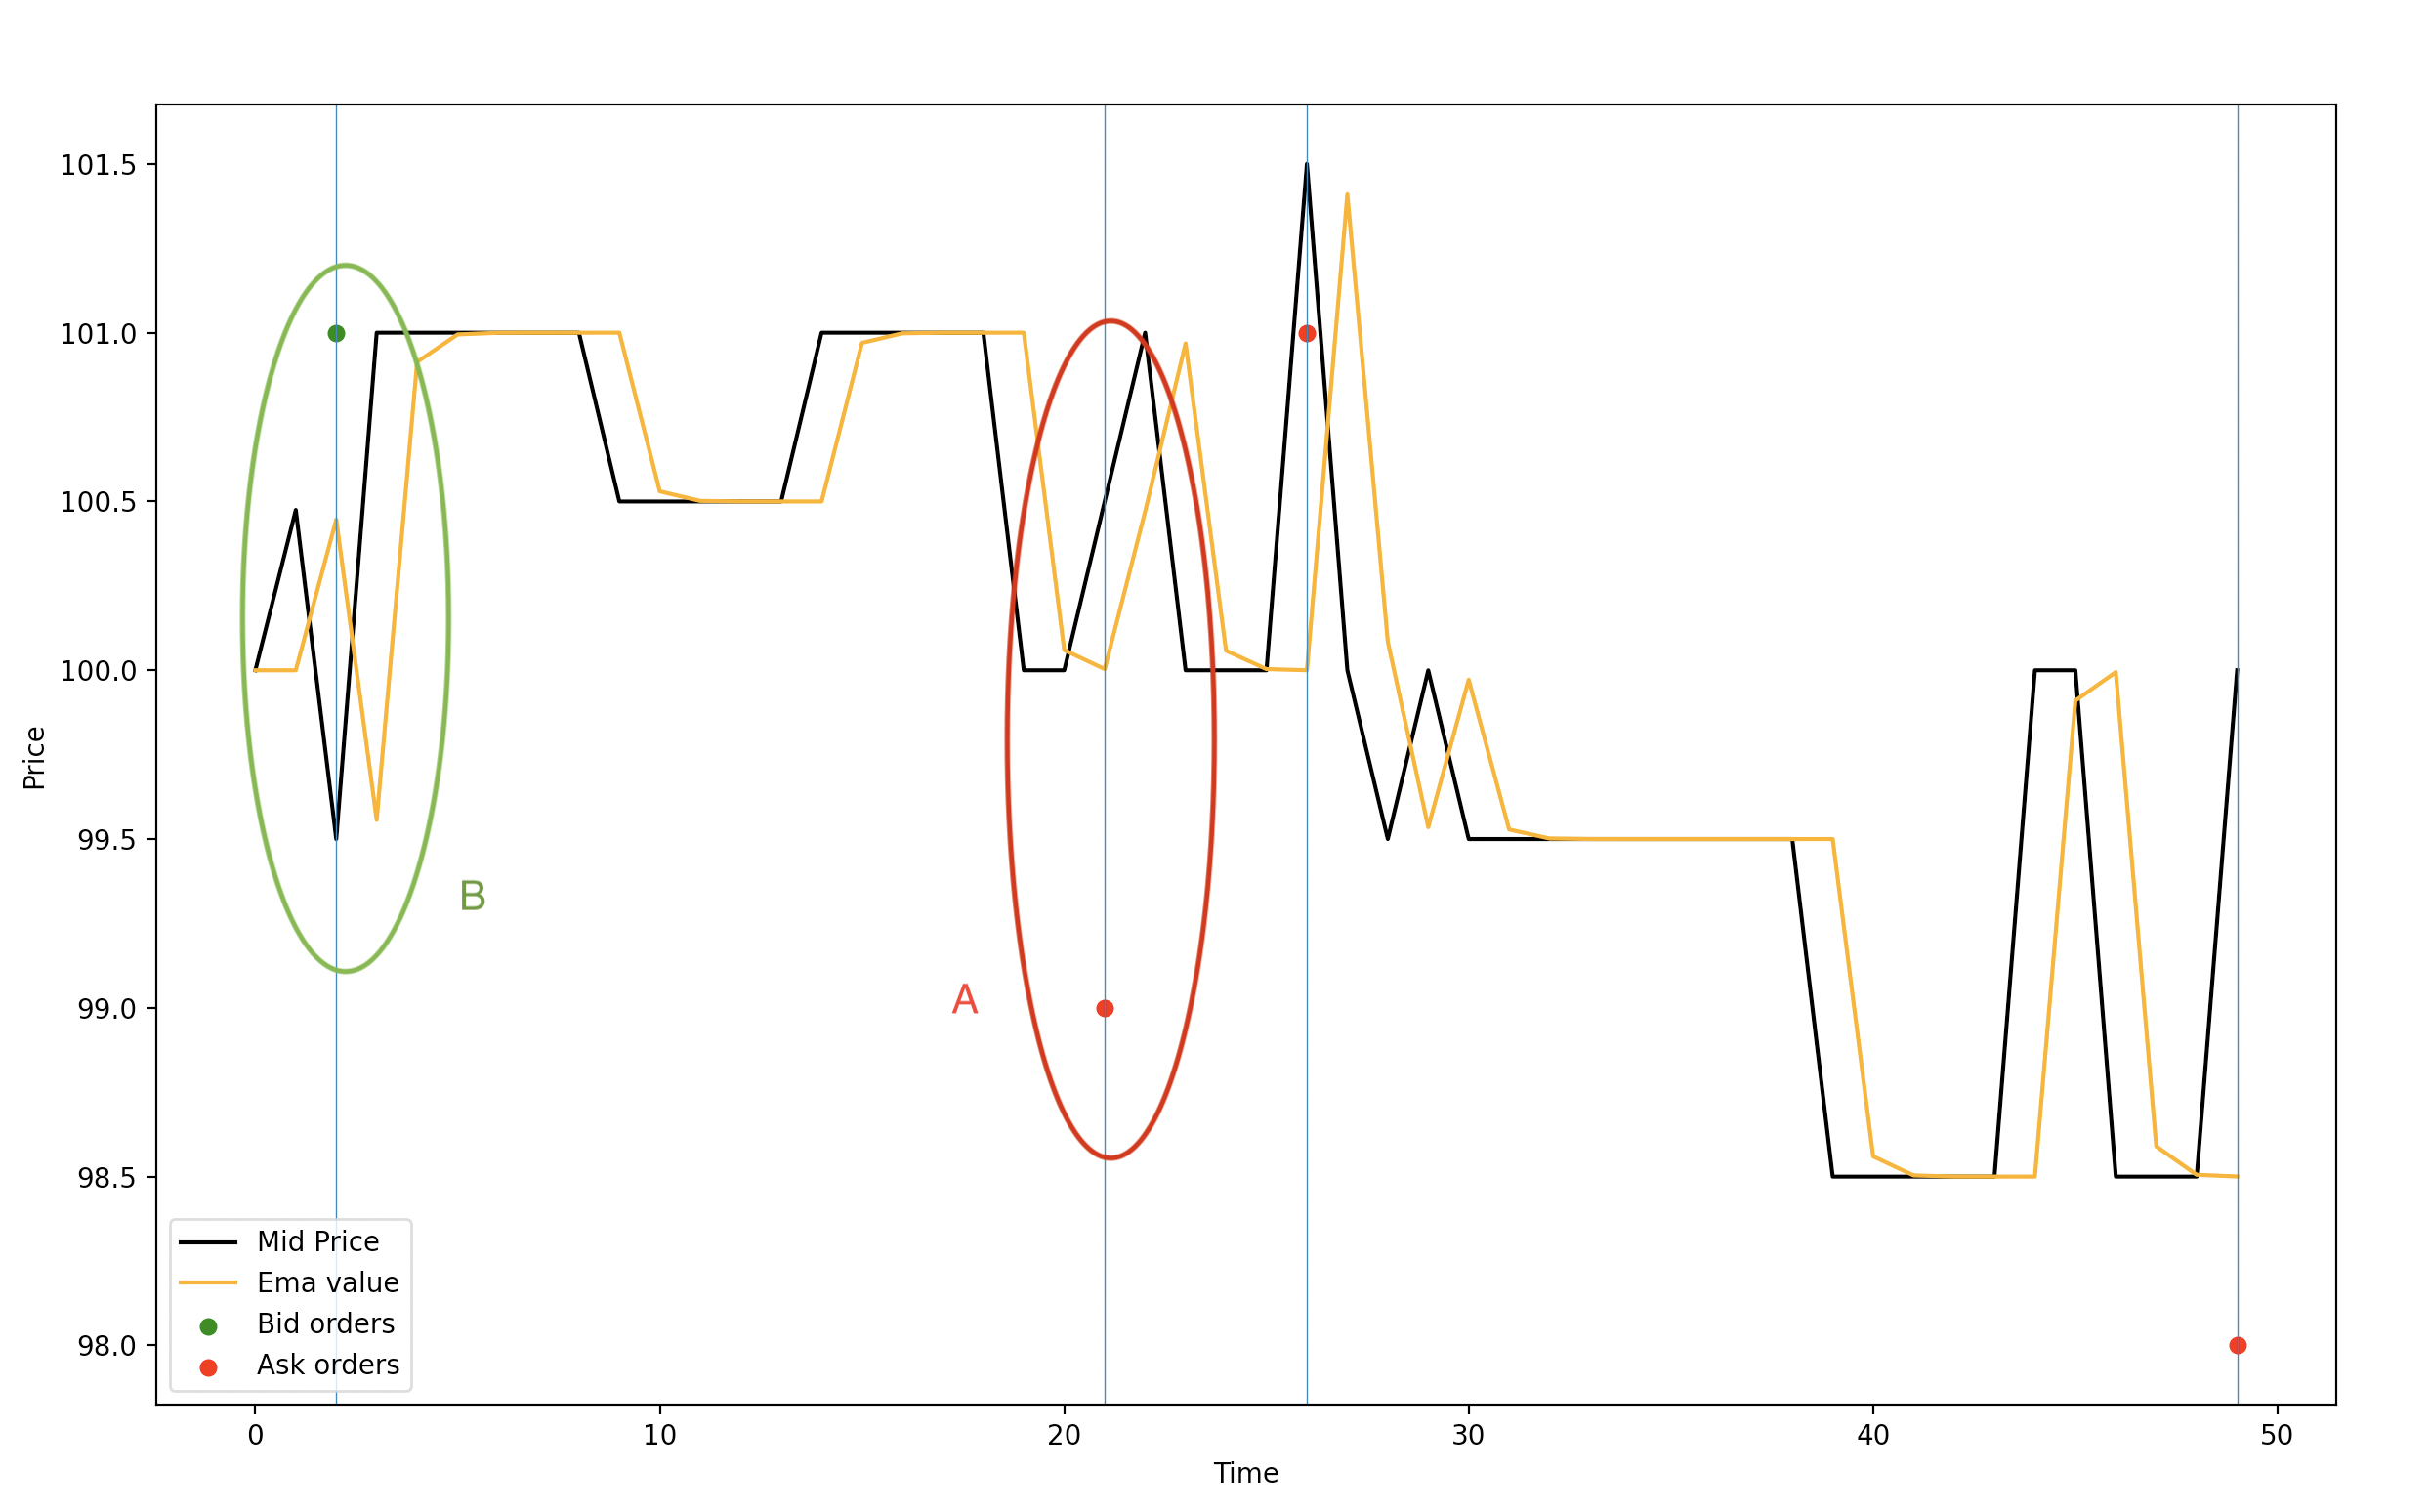
\includegraphics[ height=8cm]{Dissertation/images/mcg_indv/MEAN_R/sample.png}
\caption{Simple Agents and Mean reversion trader Experiment} 
\label{fig:MR_first_test}
\end{figure} 
\FloatBarrier

The behaviour of the Mean reversion trader can be illustrated by the three points depicted in Figure \ref{fig:MR_first_test}. 
\begin{itemize}
  \item \textbf{A} : This depict a point where the $ema_{t}$ value is below the mid price. This means that the mean reversion trader will submit an ask order because it believes that the price will eventually go down or return to the moving average. The red dot at the lower peak of the point illustrates an ask order submitted at the best ask price. This illustrates the first condition of the algorithm 4.4. We have that the $ema_{t}$ is 100 and $p_t$ is 100.5. Given that $ema_t \leq p_t$ and $k$ is 1 and the standard deviation at time t is 0.47, $0.5 \ge 1 * 0.47$, which is why the agent submitted a sell order.
  
  \item \textbf{B} : This depict a point where the $ema_{t}$ value is above the mid price. This means that the mean reversion trader will submit a bid order because it believes that the price will eventually go up back to the moving average. The green dot at the top of the point illustrates a bid order submitted at the best bid price. This illustrates the second condition of the algorithm 4.4. We have that the $ema_{t}$ is 100.5 and mid price is 99.5. The standard deviation at time t is 0.5. Given that $ema_t \ge p_t$ and and $k = 1$, we have that $1.0 \ge 0.5$, hence the agent submitted a buy order. 
  
\end{itemize}

However, this also represents a problem. The $ema_{t}$ line is not similar to what is commonly see in other literature. We have decided to test another ema equation. 

\begin{equation}
ema_t = (p_{t} - ema_{t-1}) * (2 / n + 1) + ema_{t-1} 
\end{equation}
where n = period.

If the McG value of 0.94 is calculated using this equation, then the period would be 1.1, which is the same as taking only the previous value into account. However, with the new equation, the coefficient will be 0.04, which is much less than the value specified in McG paper. 

\begin{figure}[h]
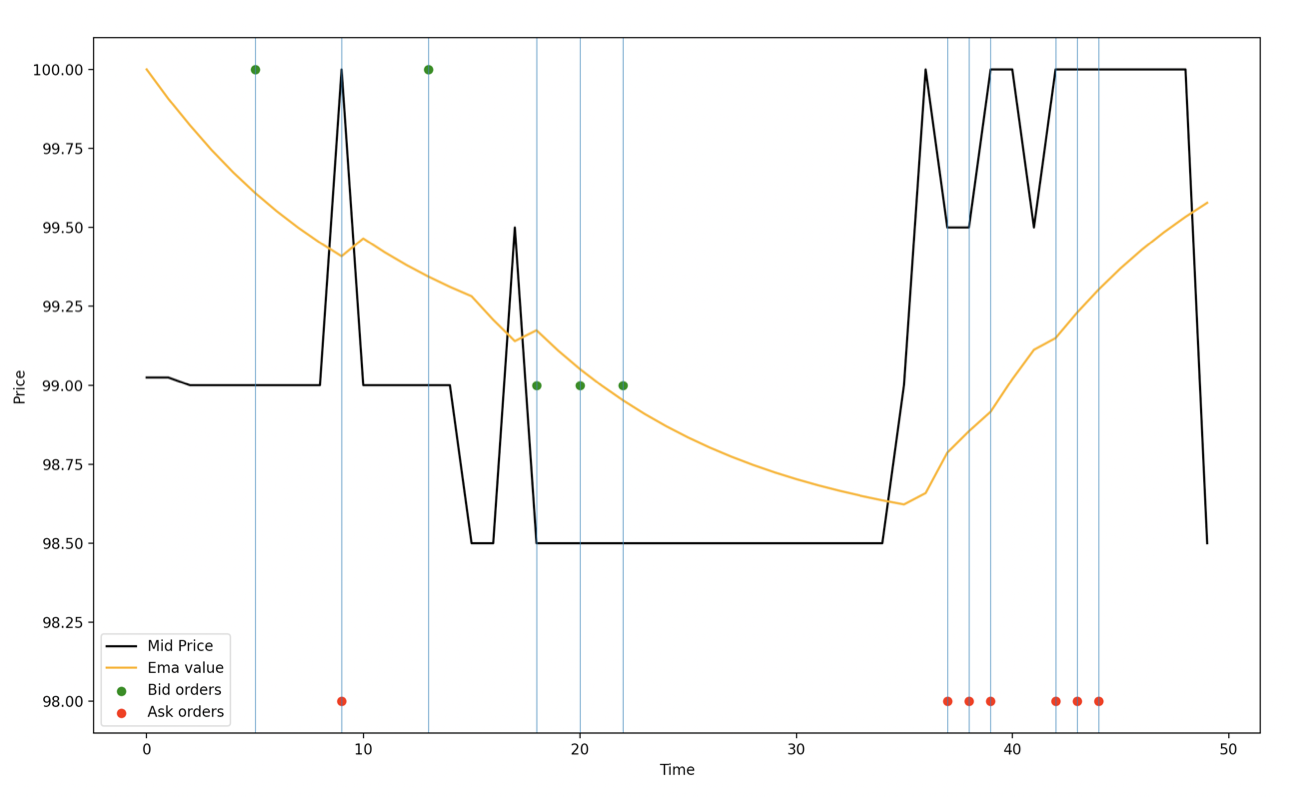
\includegraphics[ height=8cm]{Dissertation/images/mcg_indv/MEAN_R/online.png}
\caption{Simple Agents and Mean reversion trader Experiment} 
\label{fig:MR_online}
\end{figure} 
\FloatBarrier

Figure \ref{fig:MR_online} illustrates the same experiment with the new $ema_t$ equation. The Mean reversion agent still submits the orders in the same behaviour but the $ema_t$ line is much similar to that of other literature. 

\section{Noise trader} 
The Noise trade is also based on Cui and Barbazon \cite{CuiNoise} conference paper. Cui and Barbazon main objective was to examine wheter intelligence in a trading agent is needed to mimic the price impact and size of order relationship, which is why they implemented the Noise trader in order to replicate the statistics seen in real financial exchange. This is why the  Noise trader is defined so that it can captures other activities in the financial market since its parameters are based on real market data. It randomly execute a sell or a buy with equal probability. Once decided, the agent either place a market order or limit order or cancel existing order with probability $\lambda_{m}$, $\lambda_{l}$ and $\lambda_{c}$ respectively. If it does submit an order, the volume is drawn from a log-normal distribution described by:
\begin{equation}
v_t = exp(\mu + \sigma u_v) 
\end{equation}
where $\mu$ and $\sigma$ is mean and standard deviation of the $v_{ts}$ natural logarithm. $u_v$ is a value uniformly drawn between 0 and 1. Two other conditions of the Noise trader is as follow: 

\begin{itemize}
    \item Noise trader's market orders quantity cannot be more than half of the opposite side of the book
    \item Noise trader must make sure no side of the book is empty and submit limit orders accordingly
\end{itemize}
\begin{algorithm}[H]
\DontPrintSemicolon 
\If{$random() < \delta_{nt}$} {

    \If{$random() < 0.5$} {
    Decides to Sell\;
    }
    \Else{
    Decides to Buy;\
    }
    \EndIf
    Generate $U(0,1)$ to determine action,$\lambda_{m}$ , $\lambda_{l}$ and $\lambda_{c}$.
    
    \Switch{action}
    {
        \Case{Submit Market Order with probability $\lambda_{m}$ }{Submit market order with volume calculated by $v_{nt} = exp(\mu + \sigma u_v)$}
        \Case{Submit Limit Order with probability $\lambda_{l}$}{
        Generate $U(0,1)$ to determine action,$\lambda_{crs}$ , $\lambda_{inspr}$,$\lambda_{spr}$  and $\lambda_{cspr}$.
            \tcc{The condition of these cases are such that $\lambda_{crs} + \lambda_{inspr} + \lambda_{spr} + \lambda_{offspr} = 1$. }
            \Switch{action}
            {
                \Case{Crossing Limit Order with probability $\lambda_{crs}$ }{Submit limit order at opposing best price with volume $v_{nt}$ }
                \Case{Inside spread limit order with probability $\lambda_{inspr}$ }{Generate random value with $U(BestBid,BestAsk)$ with volume $v_{nt}$}
                \Case{Spread Limit Order with probability $\lambda_{spr}$ }{Submit limit order at the best price with volume $v_{nt}$}
                \Case{Off-spread Limit Order with probability $\lambda_{offspr}$ }{Generate a random price value using $xmin_{offspr} * (1-u_0)^{-\frac{1}{\beta - 1}}$ with volume $v_{nt}$ }
            
            }
        }
        \Case{Cancel Existing Order with probability $\lambda_{c}$ }{Cancel the oldest order previously submitted.}
    }
  }
\EndIf
\caption{{\sc Noise trader reproduced from McG (4.5) \cite{McGroarty}} }
\end{algorithm}

\begin{table}[h]
\centering
\begin{tabular}{ |m||p{4cm}|} 
\hline
\textbf{Noise Trader Parameters}& \textbf{Value} \\
\hline
\hline
buy or sell & $ p_{action} = 0.5 $ \\ 
\hline
Market order probability & $\lambda_{m}$ = 0.03\\ 
\hline
Limit order probability & $\lambda_{l}$ = 0.54\\ 
\hline
Cancel order probability & $\lamda_{c}$ = 0.43\\
\hline 
Market order quantity & $\mu_{mo} = 7 \sigma_{mo} = 0.1 $\\
\hline
Limit Order quantity &  $\mu_{lo} = 8 \sigma_{lo} = 0.7 $\\
\hline
Off-spread relative price & $xmin_{offspr} =0.005$
\newline 
$\beta_{offspr} = 2.72 $\\
\hline
\textbf{Limit order types} & \\
\hline
Crossing limit order & $\lamda_{crs} = 0.003$\\
\hline 
Inside-spread Limit order & $\lamda_{inspr} = 0.098$\\
\hline 
Spread Limit order & $\lamda_{spr} = 0.173$\\
\hline 
Off-spread Limit order & $\lamda_{offspr} = 0.726$\\
\hline
\end{tabular}
\caption{Noise trader parameters taken from \cite{McGroarty}}
\end{table}
\FloatBarrier 

The Noise trader is intended to represent other forms of behaviour in the market. By looking at the parameters of the Noise trader, it is clear that the Noise agent will mostly either submit a limit order or cancel an order. By taking a closer look at the limit order, the agent will mostly submit an Off-spread limit order. According to Cui and Barbazon \cite{CuiNoise}, the Off-spread price of the order is given by the $BestBid - RP_{offspr}$ in a bid order and $BestAsk + RP_{offspr}$ in an ask order. The value $RP_{offspr}$ is given by $xmin_{offspr} * (1-u_0)^{-\frac{1}{\beta - 1}}$. This is equivalent to the price below the Best Bid and above the Best Ask.

By looking the values of the $RP_{offspr}$, one can predict what the range of the price submitted can be. 

\begin{table}[h]
\centering
\begin{tabular}{ |m||p{4cm}|} 
\hline
\textbf{Uniform random value $u_0$}& \textbf{$RP_{offspr}$ Value} \\
\hline
\hline
0 & 0.5\\
\hline 
0.1 & 0.5\\
\hline 
0.2 & 0.4\\
\hline 
0.3 & 0.4\\
\hline 
0.4 & 0.4\\
\hline 
0.5 & 0.3\\
\hline 
0.6 & 0.3\\
\hline 
0.7 & 0.2\\
\hline 
0.8 & 0.2\\
\hline 
0.9 & 0.1\\
\hline 
1.0 & 0.0\\
\hline
\end{tabular}
\caption{Noise trader parameters taken from \cite{McGroarty}}
\end{table}
\FloatBarrier 

Table 4.6 of $RP_{offspr}$ calculations illustrates how the values of the off-spr price should not vary much from the initial price. Figure \ref{fig:Noise_test_mp} below illustrates that price that the Noise trader submits within a market of homogeneous 6 Noise agents running with 3000 McG time-period or ten-percent of the whole run-time. The initial price is 100 and the spread is 0.5. 

\begin{figure}[!htbp]
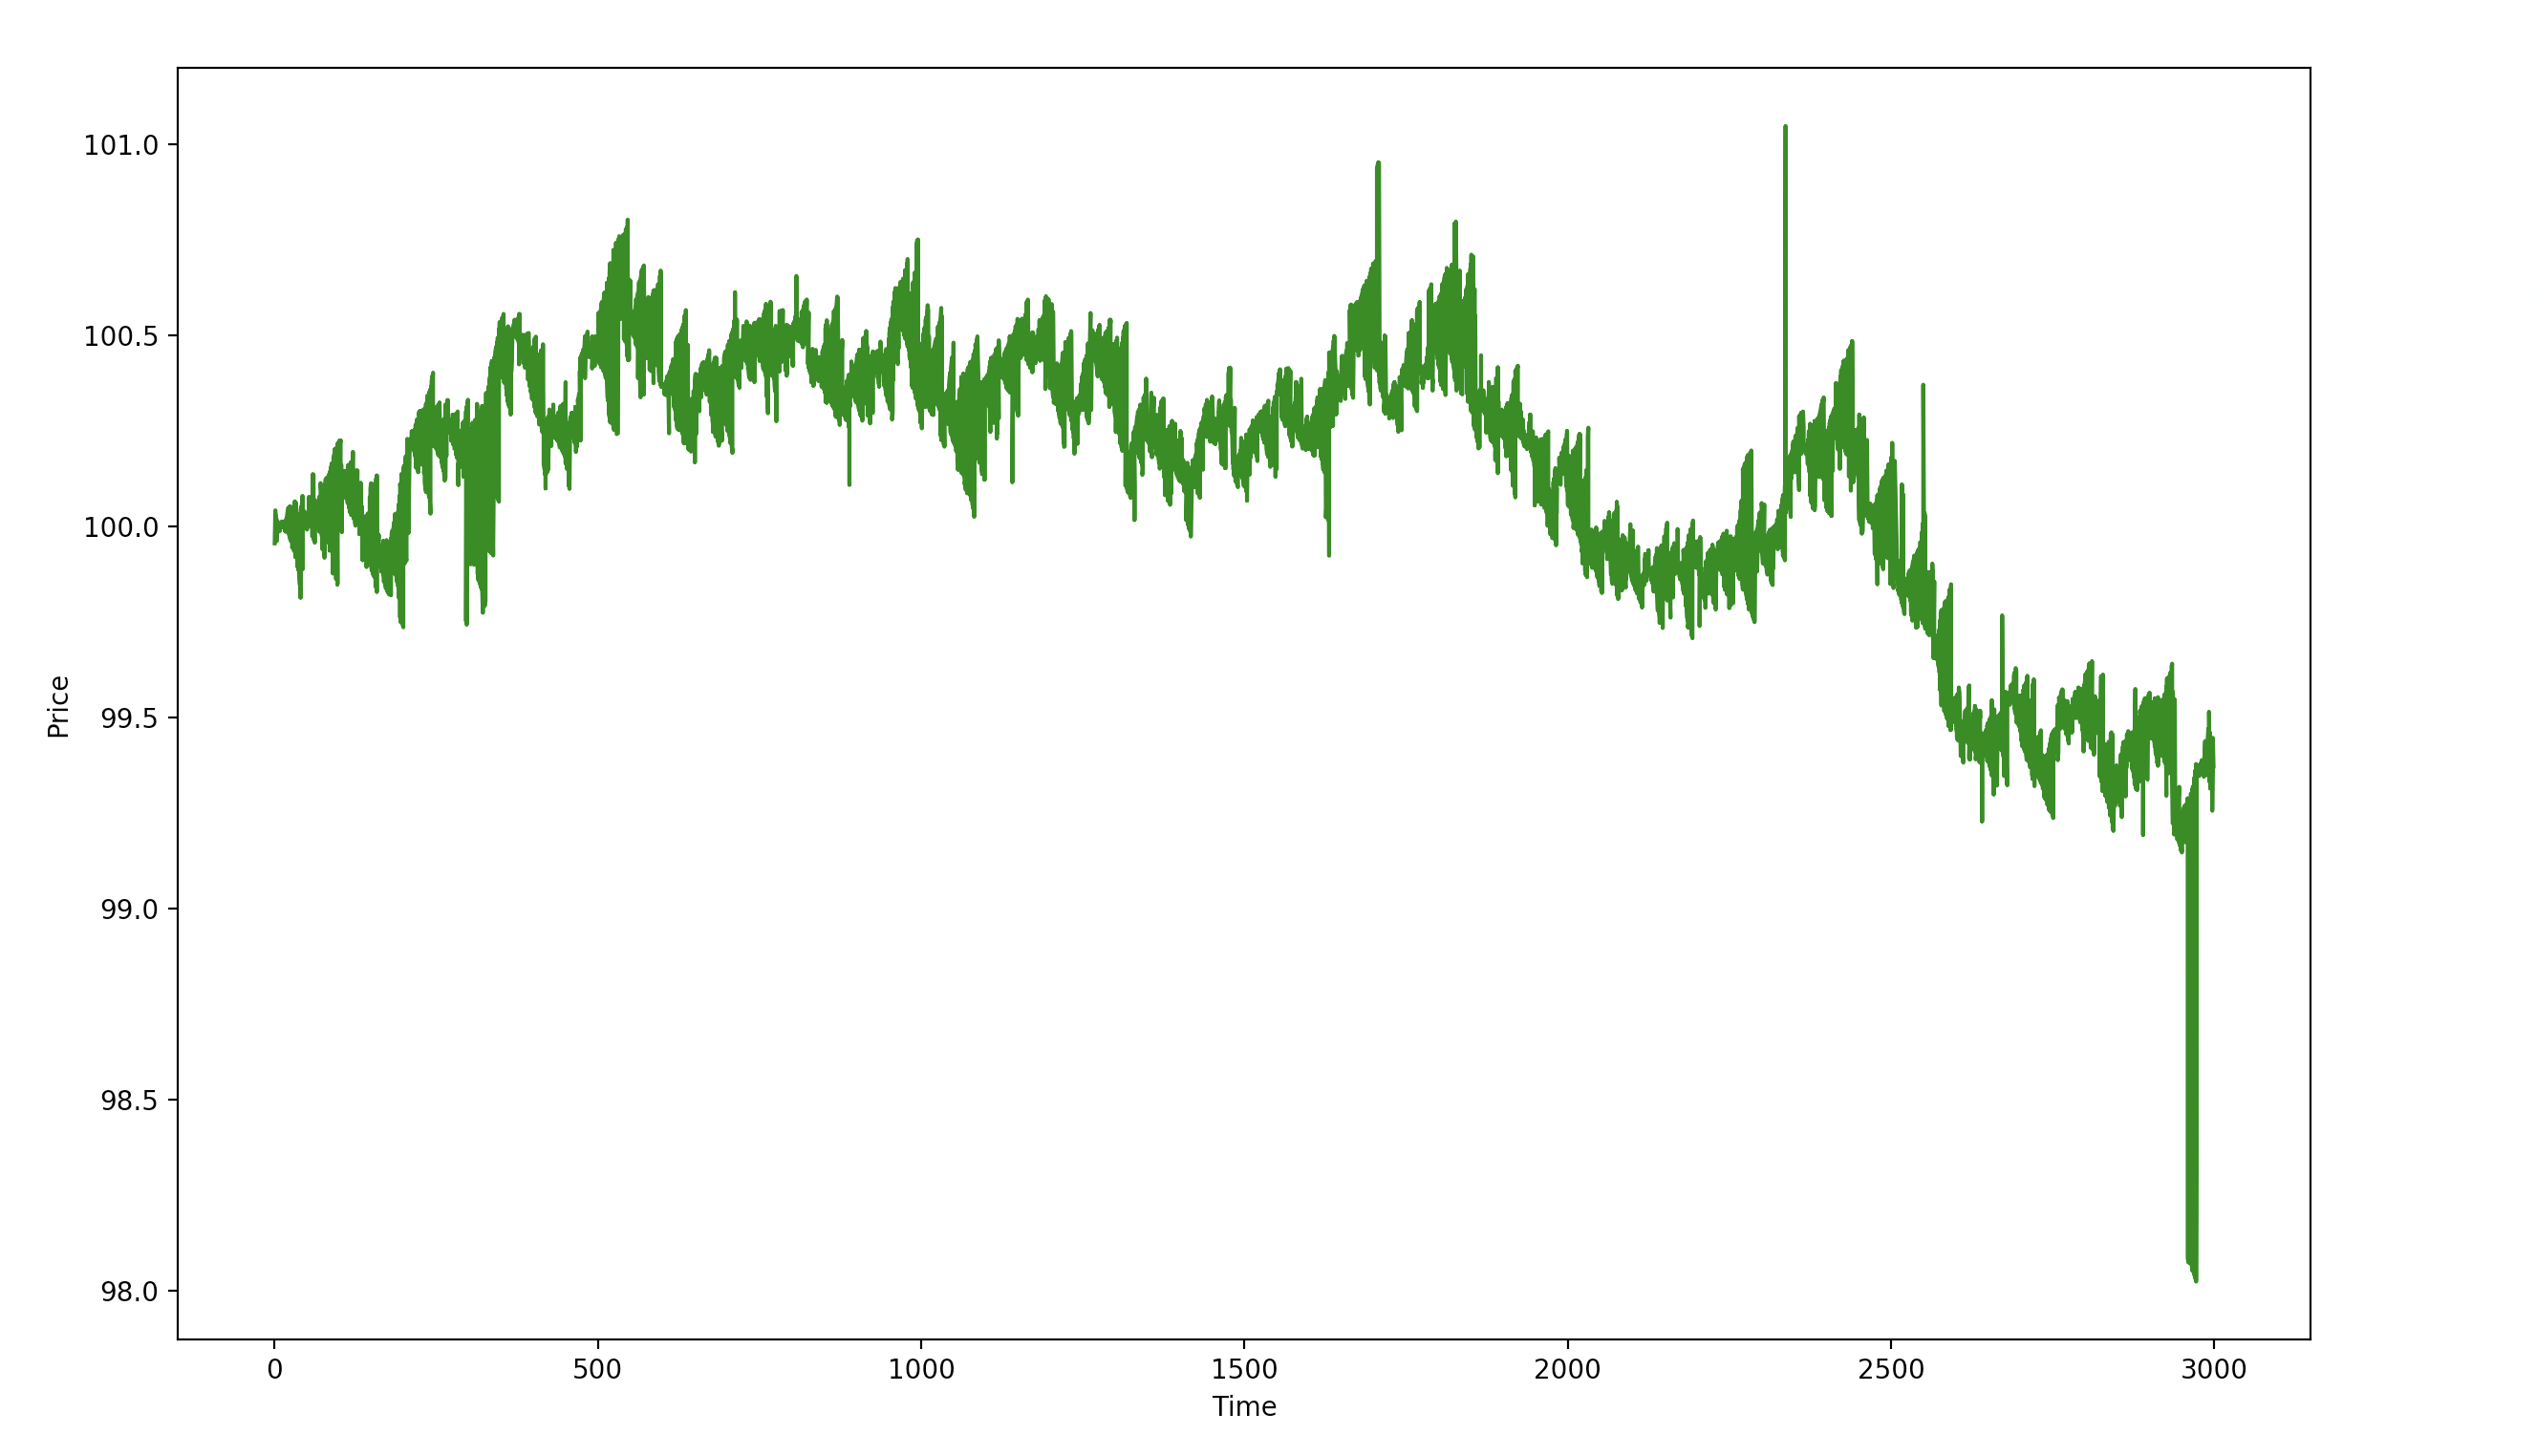
\includegraphics[ height=8cm]{Dissertation/images/mcg_indv/Screenshot 2020-03-20 at 14.33.18.png}
\caption{Noise trader order price} 
\label{fig:Noise_test_mp}
\end{figure} 
\FloatBarrier

 
As expected, the price is hugely volatile, due to the random variable of the off-spread price and inside spread limit order. However, the range is still near the initial price and gradually decreases due to the sudden decrease by 0.5 from the off-spr price, which is what can be expected. 

\subsection{Limit Order prices}
In this section, the purpose is do demonstrate the price ranges that the Noise trader will submit in its limit orders.

\begin{algorithm}[H]
\DontPrintSemicolon 
\Switch{action}
            {
                \Case{Crossing Limit Order }{Submit limit order at opposing best price with volume $v_nt$ }
                \Case{Inside spread limit order }{Generate random value with $U(BestBid,BestAsk)$ with volume $v_nt$}
                \Case{Spread Limit Order }{Submit limit order at the best price with volume $v_nt$}
                \Case{Off-spread Limit Order }{Generate a random price value using $xmin_{offspr} * (1-u_0)^{-\frac{1}{\beta - 1}}$ }
            
            }
\caption{{\sc Noise trader Limit order algorithm reproduced from McG (4.5) \cite{McGroarty}}}
\end{algorithm}

In this experiment, the market will consist of 10 Noise traders, running for 30,000 McG time-step to demonstrate the price ranges. For simplicity, we will set the best ask to 299 and best bid to 301 in order to see the variations in order prices and not the best prices itself. The results are given below. 

\begin{table}[h]
\centering
\begin{tabular}{ |l||l|l|l|} 
\hline
\textbf{Order type}& \textbf{Probability} & \textbf{Min value} & \textbf{Max value} \\
\hline
\hline
Crossing Limit order & 0.003 & 299 & 301 \\ 
\hline
Inside spread Limit order & 0.098 & 299 & 300.99 \\ 
\hline
Spread Limit order & 0.173 & 299 & 301 \\ 
\hline
Off-spread Limit order & 0.726 & 299.00& 300.99 \\ 
\hline
\end{tabular}
\caption{Number of transactions in each implementation}  
\end{table}
\FloatBarrier

The Cross limit order, Inside spread limit order, Off-spread limit order and Spread limit order must be inside the best ask and best bid range, which in this case, it is. 

\subsection{Order types submitted overall}

In this section, the purpose is to explored how many orders are actually submitted by the Noise trader and to prove that the types of orders submitted lines up with the initial parameter of the Noise trader. 

\begin{table}[h]
\centering
\begin{tabular}{ |l||l|p{2cm}|p{6cm}|} 
\hline
\textbf{Order types} & \textbf{Probability} & \textbf{Value from Experiment} & \textbf{Rough sketch of calculation} \\
\hline
\hline
Ask order & 0.5 & 4877 & $(9284 + 554) / 2 = 4919 \approx 4877$\\ 
\hline
Bid order & 0.5 & 4961 & $(9284 + 554) / 2 = 4919 \approx 4919$\\ 
\hline
\hline
Market order & 0.03 & 554 & $(9284 + 554 + 8162) * 0.03 = 540 \approx 554$\\ 
\hline
\hline
Limit order & 0.54 & 9284 & $(9284 + 554 + 8162) * 0.54 = 9720$  
\newline $\approx 9284 $\\ 
\hline
Crossing Limit Order & 0.003 & 26 & $9284 * 0.003 = 28 \approx 26 $\\ 
\hline
Inside-spread Limit Order & 0.098 & 901 & $9284 * 0.098 = 909 \approx 901 $\\ 
\hline
Spread Limit Order & 0.173 & 1709 & $9284 * 0.173 = 1606 \approx 1709 $\\ 
\hline
Off-spread Limit Order & 0.726 & 6648 & $9284 * 0.726 = 6740 \approx 6648 $\\ 
\hline
\hline
Cancel existing order & 0.43 & 8162 & $(9284 + 554 + 8162) * 0.43 = 7740  \approx 8162 $\\ 
\hline
\end{tabular}
\caption{Noise trader experiment statistics} 
\end{table}
\FloatBarrier 

In most cases, the results line up with the statistics shown as well as the proportion of the orders types submitted.

\section{Evaluation}
This chapter provides us with a deeper insight and parameters exploration that will aide us in the market experiments in the next chapters. Overall, the agents are functioning properly and the behaviour of the agents matches what is described in McG. This means that the next step of the project is to look at how these agents behave when they act in the same market and what are the characteristics of the market which mimics that of real financial exchange market dynamics. We will first investigate the same configuration as Oesch to ensure that three out of five agents are functioning in an appropriate manner before moving to two of the remaining agents. 